
\documentclass[12pt]{article}
% \documentclass{report}
% \documentclass[journal]{IEEEtran}

\usepackage{cite}
\usepackage{amsmath,amssymb,amsfonts}
\usepackage{algorithmic}
\usepackage{graphicx}
\usepackage{textcomp}
\usepackage{bm}

\usepackage[retainorgcmds]{IEEEtrantools}


\title{Bayesian Learning using a Non-Informative Prior over Finite-Dimensional Spaces}
\author{Paul Rademacher}
%\date{}


%\graphicspath{ {C:/Users/Paul/Documents/PhD/Dissertation/Documentation/Figures/} }
\graphicspath{ {Figures/} }

\DeclareMathOperator*{\argmin}{arg\,min}
\DeclareMathOperator*{\argmax}{arg\,max}
%\DeclareMathOperator*{\nbar}{\bar{\bm{\mathrm{n}}}}


\begin{document}

\maketitle

PGR: RECONSIDER my vs y notation??? May conform better with continuous IO variables.

\section{Introduction}


This report details a Bayesian perspective on stastical learning theory when both the input and outputs exist in finite dimensional spaces and a uniform prior distribution is used. To simplify the presentation, the first sections will assume that the predictions are not driven by any observable variable; subsequently, the results will be extended to the more practical case where we want to generate an estimate given observed data.

While the validity of Bayesian methods for statistical signal processing and machine learning has long been contended, the author believes it to be a justified approach that does not necessarily imply that the generative model is `random'; rather, it simply reflects the desire of the user to formulate risk as a weighted sum of learner performance across the space of models. 

The uniform, or `non-informative', prior is of specific interest because it reflects the user's lack of confidence that his/her data was generated using any specific distribution. Integrating a learner's risk with such a prior provides a Bayesian analogy to the ``No Free Lunch'' theorem; however, it will be shown that for a general loss metric, all learning functions \emph{do not} provide the same performance.

After examining the joint and conditional probability mass functions for the unobserved outputs and the training data, the results will be applied to two of the most common loss functions in machine learning: the squared error loss function (common for regression), and the 0-1 loss function (common for classification). Optimal learners will be presented and the loss as a function of space dimensions and volume of training data will be provided. Additionally, asymptotic results for these values will be discussed to provide insight into how well these learners perform for infinite input-output spaces and as the number of training examples increases. 




\section{Basic Model}


\subsection{Objective and Bayesian Interpretation}

In this simplified treatment, we want to design a learner whose performance is measured relative to an unobserved ``output'' variable $\mathrm{y} \in \mathcal{Y} = \{ y_1, \ldots, y_M \}$. To generate a decision, the learning function uses $N$ observed training examples $\mathrm{D} \in \mathcal{D} = \mathcal{Y}^N$. It is assumed that the output and training data are independently and identically distributed according to an unknown probability mass function (PMF), 

\begin{equation}
\bm{\theta} = \begin{bmatrix} \theta_1 \\ \vdots \\ \theta_M \end{bmatrix} \in \bm{\Theta} 
= \left\{ \bm{\theta} \in {\mathbb{R}^+}^M: \sum_{m=1}^M \theta_m = 1 \right\} \;,
\end{equation}

such that,

\begin{equation}
\text{P}(y,D | \bm{\theta}) = \text{P}(y | \bm{\theta}) \prod_{n=1}^N \text{P}(D(n) | \bm{\theta}) \;,
\end{equation}

where,

\begin{IEEEeqnarray}{C}
\text{P}_{\mathrm{y}}(y_m|\bm{\theta}) = \text{P}(\mathrm{y} = y_m | \bm{\theta}) = \theta_m \;, \\
\text{P}_{\mathrm{D}(n)}(y_m|\bm{\theta}) = \text{P}(\mathrm{D}(n) = y_m | \bm{\theta}) = \theta_m \;.
\end{IEEEeqnarray}

Our objective is to create a learning function $f: \mathcal{Y}^N \mapsto \mathcal{H}$, where the codomain is the decision space, that minimizes a chosen risk functional $\mathcal{R}(f) \in \mathbb{R}^+$.  The algorithm designer makes two decisions regarding how risk is calculated. First, he/she chooses a loss function $\mathcal{L}: \mathcal{H} \times \mathcal{Y} \mapsto \mathbb{R}^+$ that assigns a penalty dependent on both the unobserved output and the decision value. Using this function, we calculate the conditional risk for a given model $\bm{\theta}$,

\begin{equation}
\mathcal{R}_{\bm{\Theta}}(f,\bm{\theta}) = \text{E}_{\mathrm{D}|\bm{\theta}} \left[ \text{E}_{\mathrm{y}|\bm{\theta}} \left[ \mathcal{L}(f(\mathrm{D}),\mathrm{y}) \right] \right] \;.
\end{equation}

Note the conditional independence between $\mathrm{y}$ and $\mathrm{D}$. The second choice the designer has is how to formulate a scalar risk from the set of conditional risks $\mathcal{R}_{\bm{\Theta}}(f,\cdot) : \bm{\Theta} \mapsto \mathbb{R}^+$. An obvious choice is to integrate over $\bm{\Theta}$; if the designer has some prior knowledge, a weighting function $w: \bm{\Theta} \mapsto \mathbb{R}^+$ can be used, such that the full risk function is,

\begin{equation}
\mathcal{R}(f) = \int_{\bm{\Theta}} w(\bm{\theta}) \mathcal{R}_{\bm{\Theta}}(f,\bm{\theta})\mathrm{d}\bm{\theta} \;.
\end{equation}

Since affine transformation of an objective function will not change its minimizer, we can freely scale the non-negative weighting function $w$ such that $\int_{\bm{\Theta}} w(\bm{\theta}) \mathrm{d}\bm{\theta} = 1$. As a result, $w$ is now a valid probability density function $\text{p}(\bm{\theta})$, allowing use of the Bayesian toolset and reducing the risk function to,   

\begin{IEEEeqnarray}{rCl}
\mathcal{R}(f) & = & \text{E}_{\bm{\theta}}\left[  \mathcal{R}_{\bm{\theta}}(f,\bm{\theta}) \right] \\
& = & \text{E}_{\mathrm{y},\mathrm{D}}\left[ \mathcal{L}(f(\mathrm{D}),\mathrm{y}) \right] \\
& = & \text{E}_\mathrm{D}\left[ \text{E}_{\mathrm{y} | \mathrm{D}} [ \mathcal{L}(f(\mathrm{D}),\mathrm{y}) ] \right] \;.
\end{IEEEeqnarray}

Now the unobserved variable $\mathrm{y}$ and the observed training data $\mathrm{D}$ are treated as jointly distributed random variables. At last, we express the optimal learning function,

\begin{equation}
f^* = \argmin_{f} \mathcal{R}(f) \;.
\end{equation}

For the general case of non-parametric learning, we place no restrictions on the achievable learning functions $f \in \mathcal{F}$. Thus, to minimize the total risk, we simply minimize the conditional expected loss given $\mathrm{D}$ for each given training set, such that,

\begin{equation} \label{f_opt_D}
f^*(\mathrm{D}) = \argmin_{h \in \mathcal{H}} \text{E}_{y|\mathrm{D}}\left[ \mathcal{L}(h,y) \right] \;.
\end{equation}

Substituting in, we find the minimum risk,

\begin{equation} \label{risk_min}
\mathcal{R}(f^*) = \text{E}_{\mathrm{D}} \left[ \min_{h \in \mathcal{H}} \text{E}_{y|\mathrm{D}}\left[ \mathcal{L}(h,y) \right] \right] \;.
\end{equation}




\subsection{Closed-forms for Select Probability Distributions}

Having formulated risk using a Bayesian treatment of the model $\bm{\theta}$, we now seek a closed form expression for the optimal learner $f^*$. From equation \eqref{f_opt_D}, we see that the learner is dependent on $\text{P}(y|D)$; this section will formulate this conditional PMF by finding $\text{P}(D)$, extending to the closely related $\text{P}(y,D)$, and them simply applying Bayes theorem.


\subsubsection{Model PDF, $\text{p}(\bm{\theta})$}

To compactly express $\text{P}(D)$, we are forced to integrate out the model parameter $\bm{\theta}$. To this end, we first elaborate on the properties of the uniform distribution $\text{P}(\bm{\theta})$. Although the previous subsection provided general equations for any model distribution $\text{p}(\bm{\theta})$, the following discussion will assume that the model distribution is uniform over $\bm{\Theta}$. Note that the probability distribution function (PDF) for $\bm{\theta}$ is degenerate, since $\text{dim}(\bm{\Theta}) < M$ . Thus, we can choose to focus exclusively on the first $M-1$ elements of $\bm{\theta}$, which we will represent as,

\begin{equation}
\bar{\bm{\theta}} = \begin{bmatrix} \theta_1 \\ \vdots \\ \theta_{M-1} \end{bmatrix} \in \bar{\bm{\Theta}} = \left\{ \bar{\bm{\theta}} \in {\mathbb{R}^+}^{(M-1)}: \sum_{m=1}^{M-1} \bar{\theta}_m \leq 1 \right\} \;.
\end{equation}

To express $\text{p}\left(\bar{\bm{\theta}}\right)$, we require a formulation of the hypervolume of set $\bar{\bm{\Theta}}$. This quantity is found in Appendix \ref{app:Theta} and allows us to provide the uniform distribution,

\begin{equation}
\text{p}\left(\bar{\bm{\theta}}\right)= (M-1)!,  \quad \forall \bar{\bm{\theta}} \in \bar{\bm{\Theta}} \;.
\end{equation}

\begin{equation}
\text{p}(\bm{\theta}) = \text{p}(\theta_M,\bar{\bm{\theta}}) = \text{p}\left( \theta_M | \bar{\bm{\theta}} \right) \text{p}\left(\bar{\bm{\theta}}\right)
= (M-1)! \cdot \delta\left( 1 - \sum_{m=1}^M \theta_m \right) \;,
\end{equation}

where $\delta(\cdot)$ is the Dirac delta function. Examples of the model PDF's are provided in Figure \ref{fig:P_theta}.

\begin{figure}
\centering
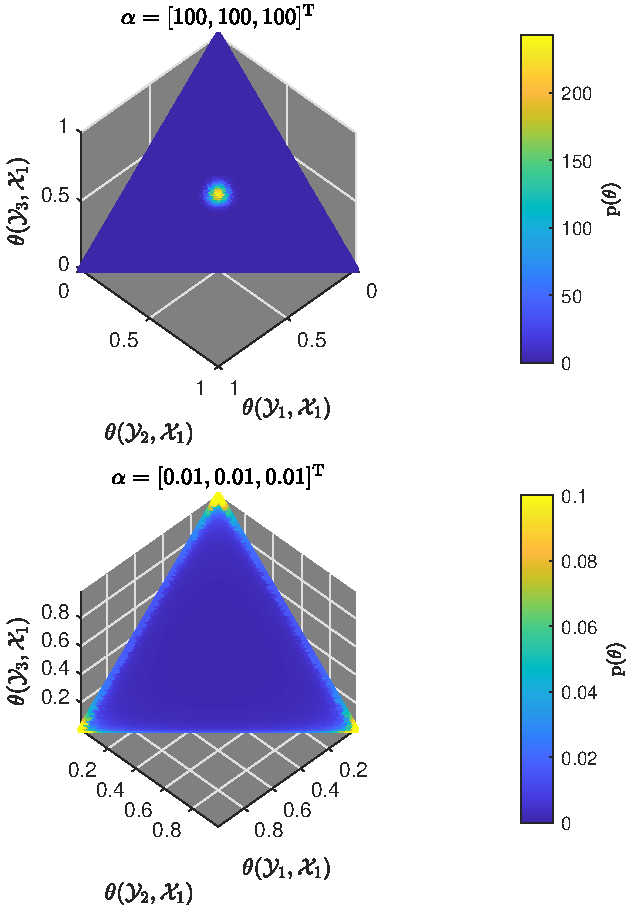
\includegraphics[scale=1.0]{P_theta.pdf}
\caption{Prior distributions for $\bar{\bm{\theta}}$ and $\bm{\theta}$, $M=3$}
\label{fig:P_theta}
\end{figure}


\subsubsection{Training data marginal PMF, $\text{P}(D)$}

Next we determine $\text{P}(D)$ -- extension to the joint distribution is straightfoward. Our starting point is expression of the PDF via the conditional independence of the training data for a given model $\bm{\theta}$,

\begin{equation}
\text{P}(D) = \int_{\bm{\Theta}} \left[ \prod_{n=1}^N \text{P}(D(n) | \bm{\theta}) \right] \text{p}(\bm{\theta}) \mathrm{d}\bm{\theta} \;.
\end{equation}

Since $\text{P}(D(n) = y_m | \bm{\theta}) = \theta_m$, we can simplify the PMF to,

\begin{equation} \label{P_D_int2}
\text{P}(D) = \int_{\bm{\Theta}} \left[ \prod_{m=1}^M \bm{\theta}_m^{\bar{N}_m(D)} \right] \text{p}(\bm{\theta}) \mathrm{d}\bm{\theta} 
= \text{E}_{\bm{\theta}} \left[ \prod_{m=1}^M \bm{\theta}_m^{\bar{N}_m(D)} \right] \;,
\end{equation}

where we have introduced a new vector random variable $\bar{\bm{\mathrm{n}}} = \bar{\bm{N}}(\mathrm{D})$ (sufficient statistic???) via transform function $\bar{\bm{N}}: \mathcal{Y}^N \mapsto \bar{\mathcal{N}} = \left\{ \bar{\bm{n}} \in \mathbb{N}^M: \sum_{m=1}^M \bar{\bm{n}}_m = N \right\}$, which is defined as,

%where we have introduced a new random variable (sufficient statistic???) $\bar{\bm{\mathrm{N}}} \in \bar{\bm{\mathcal{N}}} = \left\{ \bar{\bm{N}} \in \mathbb{N}^M: \sum_{m=1}^M \bar{\bm{N}}_m = N \right\}$ via transform function $\bar{\bm{N}}: \mathcal{Y}^N \mapsto \left\{ \bar{\bm{N}}??? \in \mathbb{N}^M: \sum_{m=1}^M \bar{\bm{N}}_m = N \right\}$, which is defined as,

\begin{equation}
\bar{N}_m(D) = \sum_{n=1}^N \delta[D(n),y_m] \;,
\end{equation}

where $\delta[\cdot,\cdot]$ is the Kronecker delta function. Observe that $\text{P}(D)$ can be interpreted as a joint moment of $\bm{\theta}$. Also, note the dimensionality reduction from $N$ to $M$ (SET SIZE???) provided by the transformation. Finally, as detailed in Appendix \ref{app:P_D}, the training data PMF reduces to,

\begin{equation} \label{P_D}
\text{P}(D) = \binom{N+M-1}{\bar{N}_1(D),\ldots,\bar{N}_M(D),M-1}^{-1} 
= \binom{N+M-1}{N,M-1}^{-1} \binom{N}{\bar{N}_1(D),\ldots,\bar{N}_M(D)}^{-1} \;.
\end{equation}

Note the use of multinomial and binomial coefficients, as well as the functional dependence on $\mathrm{D}$ only through $\bar{\bm{N}}$. It should be clear that since the PDF is inversely proportionate to the multinomial coefficient of $\bar{\bm{N}}$, training data sets are more probable when they are more ``concentrated''. 





\subsubsection{Output conditional PMF, $\text{P}(y | D)$}

Equation \eqref{P_D} can be used to illuminate the forms of all the PMF's of interest, namely $\text{P}(y)$, $\text{P}(y,D)$, and $\text{P}(y | D)$.  $\text{P}(y)$ follows immediately by evaluating $\text{P}(D)$ for $N=1$, leading to a uniform PMF,

\begin{equation}
\text{P}(y_m) = \text{E}[\theta_m] = M^{-1}, \qquad m=1,\ldots,M \;.
\end{equation}

The joint distribution between $\mathrm{y}$ and $\mathrm{D}$ is expressed by simply extending $\text{P}(D)$ to $N+1$ data and treating $y$ separately in the multinomial coefficient:

\begin{equation} \label{P_yD}
\text{P}(y_m,D) = \binom{N+M}{\ldots,\bar{N}_{m-1}(D),\bar{N}_m(D)+1,\bar{N}_{m+1}(D),\ldots,M-1}^{-1} \;.
\end{equation}

Combining previous results, the PMF of the unobserved output conditioned on the training set is,

\begin{equation} \label{P_y_D_basic}
\text{P}(y_m | D) = \frac{\text{P}(y_m,D)}{\text{P}(D)} = \frac{\bar{N}_m(D)+1}{N+M} \;.
\end{equation}

A more interesting form for the conditonal PMF is,

%\begin{equation} \label{P_y_D}
%\text{P}(y_m | D) = \left(\frac{M}{N+M}\right) M^{-1} + \left(\frac{N}{N+M}\right) \frac{\bar{N}_m(D)}{N} \;.
%\end{equation}

\begin{IEEEeqnarray}{rCl} \label{P_y_D}
\text{P}(y_m | D) & = & \left(\frac{M}{N+M}\right) M^{-1} + \left(\frac{N}{N+M}\right) \frac{\bar{N}_m(D)}{N} \\
& = & \left(\frac{M}{N+M}\right) M^{-1} + \left(\frac{N}{N+M}\right) N^{-1}\sum_{n=1}^N \delta[D(n),y_m] \;.
\end{IEEEeqnarray}

FIGURE EXAMPLE???

Observe how the terms in parentheses act as weighting factors providing a convex combination of two distributions: a uniform distribution independent of the data (specifically, $\text{P}(y_m) = \text{E}[\theta_m]$) and an empirical distribution independent of any prior knowledge.

The asymptotic behavior of this conditional PMF if of specific interest. As the cardinality $|\mathcal{Y}| = M$ increases relative to the number of training samples $N$, the PMF trends towards a uniform, ``uninformative'' distribution. Conversely, as the number of training points increases towards infinity, the PMF trends towards the empirical distribution. 






\subsubsection{Model Posterior, $\text{P}(\bm{\theta} | D)$}

Although we have already found the posterior PMF $\text{P}(y | D)$ via Bayes theorem, it is informative to consider another approach using a ``hidden'' distribution: the model posterior PDF, $\text{p}(\bm{\theta} | D)$. 

As mentioned previously, $\mathrm{y}$ and $\mathrm{D}$ have the property of conditional independence given the model; as such, $\text{P}(y,D) = \text{E}_{\bm{\theta}} \left[ \text{P}(y | \bm{\theta}) \text{P}(D | \bm{\theta}) \right]$. This enables the following interpretation of the PMF of $\mathrm{y}$ conditioned on the observed training data:

\begin{equation}
\text{P}(y_m | \mathrm{D}) = \text{E}_{\bm{\theta} | \mathrm{D}} \left[ \text{P}(y_m|\bm{\theta}) \right] = \text{E}\left[ \theta_m | \mathrm{D} \right] \;.
\end{equation}

As such, the posterior PMF $\text{P}(y | D)$ can we thought of as the expected value of $\bm{\theta}$ given the training data. This should be intuitively satisfying -- before observing the training set, the PMF of $y$ is simply $\text{E}[\bm{\theta}]$; the observations simply refine the distribution of the unknown model. Using previous results, we express the model posterior PMF in closed form as shown below. Graphical examples are provided in Figure \ref{fig:P_theta_D}.

\begin{equation} \label{P_t_D}
\text{p}(\bm{\theta} | D) = \frac{\text{P}(D | \bm{\theta}) \text{p}(\bm{\theta})}{\text{P}(D)}
= (N+M-1)! \prod_{m=1}^M \frac{\theta_m^{\bar{N}_m(D)}}{\bar{N}_m(D)!} ,  \quad  \forall \bm{\theta} \in \bm{\Theta} \;.
\end{equation}


In the machine learning literature, the model posterior is of specific interest. A popular use of the distribution is to form a point estimate of the model $\bm{\theta}$ by finding the maximizing value of the distribution - the resultant estimate is known as the Maximum \emph{a posteriori} (MAP) estimate. 

As shown in Appendix \ref{app:MAP_theta}, the MAP estimator is,

\begin{equation}
\hat{\bm{\theta}}_{MAP}(D) = \argmax_{\bm{\theta} \in \bm{\Theta}} \text{P}(\bm{\theta} | D) = \frac{\bar{\bm{N}}(D)}{N} \;,
\end{equation}

which is the same empirical distribution seen in equation \eqref{P_y_D}. Additionally, because $\text{P}(\bm{\theta})$ is uniform, the MAP estimator is equivalent to the Maximum Likelihood (ML) estimate $\hat{\bm{\theta}}_{ML}(D) = \argmax_{\bm{\theta} \in \bm{\Theta}} \text{P}(D | \bm{\theta})$, which is commonly used for non-Bayesian treatments of parameter estimation.


Next, we will provide the first and second moments of the conditional distribution and give some informative examples to show how the training data ``sharpens'' the non-informative distribution $\text{p}(\bm{\theta})$. Using equations \eqref{P_y_D_basic} and \eqref{P_y_D}, we can compactly display the mean of $\text{p}(\bm{\theta} | D)$ as,

\begin{equation}
\mu_{\bm{\theta} | D} \equiv \text{E}[\bm{\theta} | D] = \frac{\bar{\bm{N}}(D)+1}{N+M} = \left(\frac{M}{N+M}\right) M^{-1} + \left(\frac{N}{N+M}\right) \frac{\bar{\bm{N}}(D)}{N} \;.
\end{equation}

The second moments are generated in Appendix \ref{app:cov_theta_D}; combining with the mean above, we find the covariance matrix of $\bm{\theta}$ given $D$,

\begin{IEEEeqnarray}{rCl} 
\Sigma_{\bm{\theta} | D} & \equiv & \text{E}_{\bm{\theta} | D} \left[ (\bm{\theta} - \mu_{\bm{\theta} | D}) (\bm{\theta} - \mu_{\bm{\theta} | D})^\text{T} \right] \\ 
& = & \frac{\text{diag}(\bar{\bm{N}}(D) + \bm{1})}{(N+M+1)(N+M)} - \frac{(\bar{\bm{N}}(D) + \bm{1}) (\bar{\bm{N}}(D) + \bm{1})^\text{T}}{(N+M+1)(N+M)^2} \;. \label{cov_theta_D}
\end{IEEEeqnarray}

Comparing the numerators and denominators in the above expression, it is clear that as the size of the training set $N$ trends toward infinity, the variance of the model trends to zero. When also considering the limiting forms of $\mu_{\bm{\theta} | D}$, we observe that the distribution converges (in mean-square??? in distribution???) to,

\begin{equation}
\text{p}(\bm{\theta} | D) \longrightarrow \delta \left( \bm{\theta} - \frac{\bar{\bm{N}}(D)}{N} \right) \;,
\end{equation}

Thus, with infinite training data, the generative model $\bm{\theta}$ can be determined precisely and used to determine the optimal learning function. 

\begin{figure}
\centering
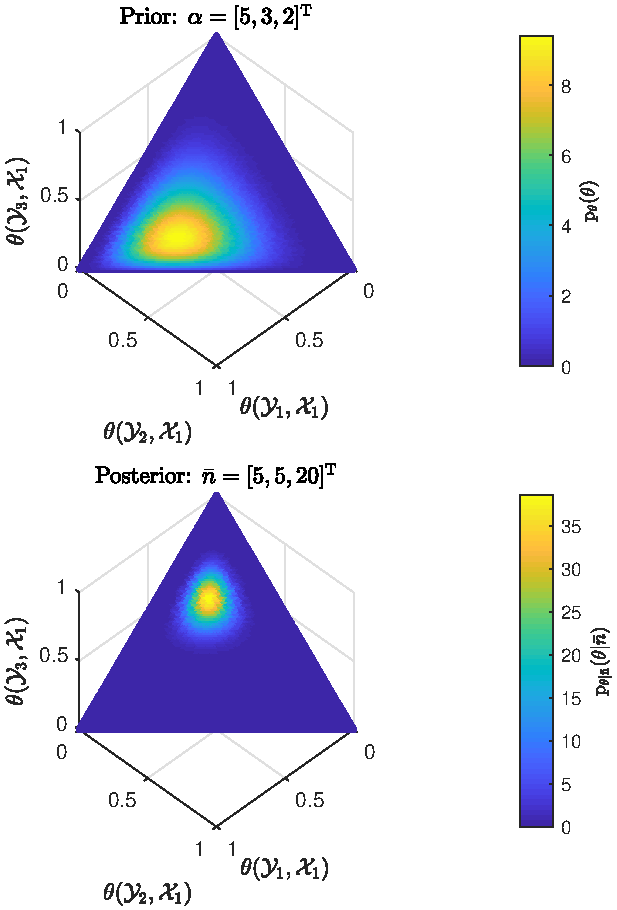
\includegraphics[scale=1.0]{P_theta_post.pdf}
\caption{Posterior model PDF's for various training sets $D$}
\label{fig:P_theta_D}
\end{figure}




\section{Application to Common Loss Functions}

In this section, we will proceed to apply the previous results to determine specific optimal learners and their performance for two of the most common loss functions in machine learning: the squared error function, common for regression problems, and the 0-1 function, common for classification problems. Noting again the significance of $\text{P}(y|D)$ in finding the optimal learner in equation \eqref{f_opt_D}, and using \eqref{P_y_D}, we have,

\begin{IEEEeqnarray}{L}
\text{E}_{\mathrm{y} | \mathrm{D}} [ \mathcal{L}(h,\mathrm{y}) ] = \sum_{m=1}^M \mathcal{L}(h,y_m) \text{P}(y_m | \mathrm{D}) \\
= \frac{\sum_{m=1}^M \mathcal{L}(h,y_m) + \sum_{n=1}^N \mathcal{L}(h,D(n))}{N+M} \\
= \left( \frac{M}{N+M} \right) \sum_{m=1}^M \mathcal{L}(h,y_m) M^{-1} +  \left( \frac{N}{N+M} \right) \sum_{m=1}^M \mathcal{L}(h,y_m) \frac{\bar{N}_m(D)}{N} \\
= \left( \frac{M}{N+M} \right) M^{-1} \sum_{m=1}^M \mathcal{L}(h,y_m) +  \left( \frac{N}{N+M} \right) N^{-1} \sum_{n=1}^N \mathcal{L}(h,D(n)) \;.
\end{IEEEeqnarray}

Note that by using the mixed distribution of \eqref{P_y_D}, we split the risk into a convex combination of two expected losses. Furthermore, by substituting in the formula for $\bar{\bm{N}}(D)$, we show the second expectation to be equivalent to the empirical loss.




\subsection{Classification: the 0-1 Loss}
In this section, we will apply the developed framework to the machine learning problem to which it is most applicable: classification. In classification problems, the unobserved variable space is countable and typically finite. Furthermore, the hypothesis space  is usually identical to the unobserved variable space, that is $\mathcal{H} = \mathcal{Y}$. The 0-1 loss function is the most well known for these problems; it is represented as,

\begin{equation} \label{loss_01}
\mathcal{L}(h,y) = 1 - \delta[h,y] \;.
\end{equation}

\subsubsection{Optimal Learner: the MAP class estimate}

To determine the optimal learning function $f$, we combine the loss function \eqref{loss_01} with the posterior PMF of equation \eqref{P_y_D_basic}; the conditional expected loss reduces to,

\begin{IEEEeqnarray}{rCl}
\text{E}_{\mathrm{y} | \mathrm{D}} [ \mathcal{L}(h_m,\mathrm{y}) ] & = & 1 - \text{P}_{\mathrm{y} | \mathrm{D}}(h_m | \mathrm{D}) \\
& = & 1 - \left( \frac{M}{N+M} \right) M^{-1} - \left( \frac{N}{N+M} \right) \frac{\bar{N}_m(D)}{N} \;.  
\end{IEEEeqnarray}

Substituting into equation \eqref{f_opt_D}, the optimal learning function can be expressed as,

\begin{IEEEeqnarray}{rCl}
f^*(\mathrm{D}) & = & \argmin_{h \in \mathcal{Y}} \text{E}_{\mathrm{y} | \mathrm{D}}\left[ 1 - \text{P}_{\mathrm{y} | \mathrm{D}}(h | \mathrm{D})  \right] \\
& = & \argmax_{h \in \mathcal{Y}} \text{P}_{\mathrm{y} | \mathrm{D}}(h | \mathrm{D}) \;,
\end{IEEEeqnarray}

or, specifically,

\begin{equation}
f^*(\mathrm{D}) = y_{m^*},  \quad \text{where } m^* = \argmax \bar{N}_m(\mathrm{D}) \;.
\end{equation}

Given our lack of prior confidence in any of the data-generating PMF's $\bm{\theta}$, the best class estimate is simply found by choosing the class most represented in the training set $D$.


\subsubsection{Minimum Risk: the Probability of Error}
Now, we determine the minimum risk (probability of error for the 0-1 loss). Starting from equation \eqref{risk_min}, we formulate the risk as,

\begin{IEEEeqnarray}{rCl}
\mathcal{R}(f^*) & = & \text{E}_{\mathrm{D}} \left[ \text{E}_{\mathrm{y} | \mathrm{D}} [ \mathcal{L}(f^*(\mathrm{D}),\mathrm{y}) ] \right]
= 1 - \text{E}_{\mathrm{D}} \left[ \max_{y} \text{P}_{\mathrm{y} | \mathrm{D}}(y | \mathrm{D}) \right] \\
& = & 1 - \text{E}_{\mathrm{D}} \left[ \frac{\max_m \bar{N}_m(D) + 1}{N+M} \right] \\\
& = & 1 - \left( \frac{M}{N+M} \right) M^{-1} - \left( \frac{N}{N+M} \right) \frac{\text{E}_\mathrm{D} \left[ \max_m \bar{N}_m(\mathrm{D}) \right]}{N} \;. \label{risk_01_opt}
\end{IEEEeqnarray}

Before refining this expression, observe how the minimum risk trends as $M$ increases for fixed training set size $N$. Clearly, $\lim_{M \to \infty} \mathcal{R}(f^*) = 1 - M^{-1}$. This should be intuitively satisfying -- the posterior PMF trends toward a discrete uniform distribution, the same as if no data had been observed at all (e.g. $\text{P}(y_m) = M^{-1}$).

Next, we continue to find a closed-form expression for the optimal risk; to do so, we must evaluate the expectation over all possible training sets $D$. It can be clearly shown that the expectation can instead be performed over random variable $\bar{\bm{\mathrm{n}}} = \bar{\bm{N}}(\mathrm{D})$, that is,

\begin{equation}
\text{E}_\mathrm{D} \left[ \max_m \bar{N}_m(\mathrm{D}) \right] = \text{E}_{\bar{\bm{n}}} \left[ \max_m \bar{\mathrm{n}}_m \right] \;.
\end{equation}

In Appendix \ref{app:E_N_max}, we determine the cumulative mass function (CMF) of $\bar{\mathrm{n}}_{\text{max}} \equiv \max_m \bar{\mathrm{n}}_m$, 

\begin{IEEEeqnarray}{rCl}
F_{\bar{\mathrm{n}}_{\text{max}}}(n) & = & \text{P}\left( \bar{\mathrm{n}}_{\text{max}} \leq n \right) \\
& = & \binom{N+M-1}{M-1}^{-1} \sum_{m=1}^M \binom{M}{m} (-1)^{M-m} \\
&& \quad \binom{m(n+1)-N-1}{M-1} U\left( n+1-\left\lceil\frac{N+M}{m}\right\rceil \right) \;.
\end{IEEEeqnarray}

where $U: \mathbb{R} \mapsto \{0,1\}$ is the continuous step function. Clearly, the PMF is zero outside of the interval $[0,N+M]$; the expected value is thus,

\begin{IEEEeqnarray}{rCl}
\text{E}_{\bar{\bm{n}}} \left[ \bar{\mathrm{n}}_{\text{max}} \right] & = & \sum_{n=0}^{N+M} n \left( F_{\bar{\mathrm{n}}_{\text{max}}}(n) - F_{\bar{\mathrm{n}}_{\text{max}}}(n-1) \right) \\
& = & N + M - \sum_{n=0}^{N+M-1} F_{\bar{\mathrm{n}}_{\text{max}}}(n) \\
& = & N + M - \binom{N+M-1}{M-1}^{-1} \sum_{m=1}^M \binom{M}{m} (-1)^{M-m} \\
&& \quad \sum_{n = \left\lceil \frac{N+M}{m} \right\rceil}^{N+M} \binom{mn-N-1}{M-1} \;.
\end{IEEEeqnarray}

This general equation has not been reduced to a more tractable form. Using it it conjunction with equation \eqref{risk_01_opt}, we have the expression for the optimal risk,

\begin{IEEEeqnarray}{rCl}
\mathcal{R}(f^*) & = & 1 - \text{E}_{\mathrm{D}} \left[ \frac{\max_m \bar{N}_m(D) + 1}{N+M} \right] \\
& = & \frac{1}{N+M} \left[ -1 + \binom{N+M-1}{M-1}^{-1} \sum_{m=1}^M \binom{M}{m} (-1)^{M-m} \sum_{n = \left\lceil \frac{N+M}{m} \right\rceil}^{N+M} \binom{mn-N-1}{M-1}  \right] \\
& = & \frac{-1}{N+M} \left[ 1 + \sum_{m=1}^M \binom{M}{m} (-1)^m \sum_{n = \left\lceil \frac{N+M}{m} \right\rceil}^{N+M} \prod_{l=1}^{M-1} \left( 1 - \frac{mn}{N+l} \right) \right] \;.
%& = & \frac{M - 1 +\binom{N+M-1}{M-1}^{-1} \sum_{m=1}^M \binom{M}{m} (-1)^{M-m} \sum_{n = \left\lceil \frac{N+M}{m} \right\rceil}^N \binom{mn-N-1}{M-1}}{N+M} \;.
\end{IEEEeqnarray}

PGR: Havent found closed form for summation over n. Can a bound be found instead???

Figure \ref{fig:Risk_01_vsN} displays the risk as a function of $N$ for select values of $M$. Observe that even for binary classification, the optimal risk asymptotes quickly.

\begin{figure}
\centering
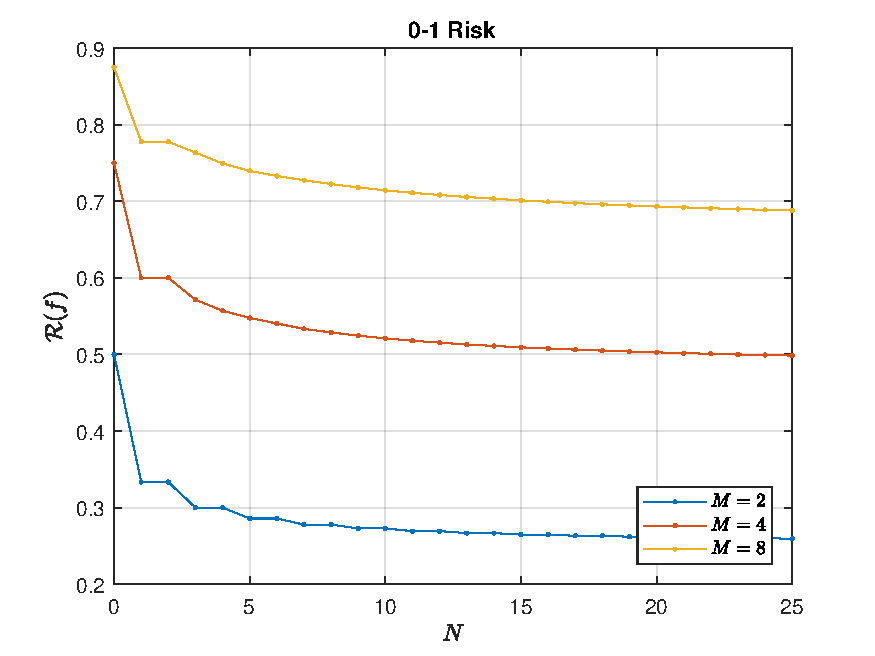
\includegraphics[scale=1.0]{Risk_01_vsN.pdf}
\caption{Optimal 0-1 Risk, vs. Training Set volume $N$}
\label{fig:Risk_01_vsN}
\end{figure}


The performance of this optimal decision function in the limit of training set volume $N \to \infty$ is of interest. Fortunately, the expectation $\text{E}_{\bar{\bm{n}}} \left[ \max_m \bar{n}_m \right]$ can be represented more compactly in this limit. As detailed in Appendix \ref{app:E_N_max},

\begin{equation}
\lim_{N \to \infty} \frac{\text{E}_{\bar{\bm{n}}} \left[ \max_m \bar{n}_m \right]}{N} = \frac{1}{M} \sum_{m=1}^M \frac{1}{m} \;.
\end{equation}

Note that this summation has no closed-form -- it is a Harmonic number (REFERENCE???) Note also that if the class set is countably infinite, this summation can be represented as,

\begin{equation}
\lim_{M \to \infty} \frac{1}{M} \sum_{m=1}^M \frac{1}{m} = \frac{\text{ln}(M)}{M} \;.
\end{equation}

Substituting the limiting form of the expectation into equation \eqref{risk_01_opt}, we determine the optimal risk,

\begin{equation}
\lim_{N \to \infty} \mathcal{R}(f^*)  = \lim_{N \to \infty} \left( 1 - \frac{\text{E}_\mathrm{D} \left[ \max_m \bar{N}_m(\mathrm{D}) \right]}{N} \right) = 1 - \frac{1}{M} \sum_{m=1}^M \frac{1}{m} \;,
\end{equation}

which provides a lower bound to the risk that any learner can achieve with any volume of training data. Figure \ref{fig:Risk_01_LB} displays this risk, as well as the optimal risk when no training data is available. Note the margin in the probability of error between the optimal $N=0$ and $N \to \infty$ learners. For binary classification (the simplest case), we see a modest reduction from 0.5 to 0.25 error; for higher values of $M$, the probability of error increases towards unity. Clearly, this level of error is unacceptable for most applications. Nonetheless, it is the minimum risk for the problem we have formulated -- this results from our choosing a non-informative prior over $\bm{\Theta}$.


\begin{figure}
\centering
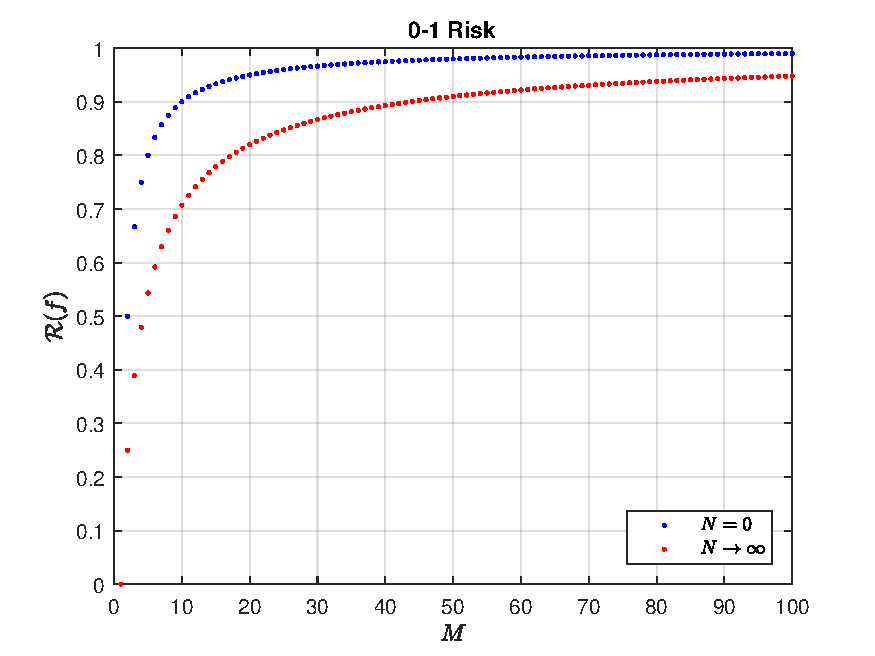
\includegraphics[scale=1.0]{Risk_01_LB.pdf}
\caption{Optimal 0-1 Risk, Upper and Lower bounds}
\label{fig:Risk_01_LB}
\end{figure}

PLOT RISK VS THETA???


\subsection{Regession: the Squared-Error Loss}

The squared-error (SE) loss function is by far the most commonly used loss function for regression, or in fact any estimation problems where the variable of interest is continuous. This is due to its convexity, which allows easy determination of the minimizing learner. 

Up until now, the $M$ elements of the unobserved output set $\mathcal{Y}$ have remained abstract, without imposing any order to the elements (besides the indexing notation). For regression, we will assign numerical values to the unobserved output; specifically, $y_m = m$, such that $\mathcal{Y} = \{1,\ldots,M\}$. Additionally, we will allow the learning function's decision to lie on the real line; thus, $\mathcal{H} = \mathbb{R} \supset \mathcal{Y}$.

The loss function is defined as,

\begin{equation}
\mathcal{L}(h,y) = (h-y)^2 \;.
\end{equation}


\subsubsection{Optimal Learner: The Posterior Mean}

To determine the optimal learning function, we expand the conditional expectation,

\begin{IEEEeqnarray}{rCl} \label{f_opt_mse}
\text{E}_{\mathrm{y} | \mathrm{D}} [ \mathcal{L}(h,\mathrm{y}) ] & = & \sum_{m=1}^M (h-m)^2 \text{P}_{\mathrm{y} | \mathrm{D}}(m) \;.
\end{IEEEeqnarray}

Clearly, this function is quadratic and thus convex over $\mathcal{H}$ -- the minimizing value is the sole stationary point. Differentiating and equating to zero, we find,

\begin{IEEEeqnarray}{rCl}
f^*(\mathrm{D}) & = & \argmin_{h \in \mathbb{R}} \text{E}_{\mathrm{y} | \mathrm{D}} \left[ (h-\mathrm{y})^2 \right] \\
& = & \sum_{m=1}^M m \text{P}_{\mathrm{y} | \mathrm{D}}(m) \equiv \mu_{\mathrm{y} | \mathrm{D}} \\
& = & \left(\frac{M}{N+M}\right) \frac{M+1}{2} + \left(\frac{N}{N+M}\right) \sum_{m=1}^M m \frac{\bar{N}_m(D)}{N} \\
& = & \left(\frac{M}{N+M}\right) \frac{M+1}{2} + \left(\frac{N}{N+M}\right) \frac{1}{N} \sum_{n=1}^N D(n) \;.
\end{IEEEeqnarray}

where we have substituted in equation \eqref{P_y_D} for the posterior PMF. Our interpretation of the posterior as a mixture distribution is notable here; the optimal learner is a convex combination of two PMF mean values. Furthermore, the second mean can be represented as the average value in the training set $\mathrm{D}$.

The mixture of moments prompts analysis of the optimal learner's asymptotic behavior. Clearly, if the unobserved variable $\mathrm{y}$ is drawn from an infinite set (e.g. $\mathbb{N}$), such that $M \to \infty$, then the minimum squared error (MSE) estimate is the average value of the set $\mathcal{Y}$ and does not depend on the training data at all. Conversely, if $M$ is finite, then as the training data volume increases, the optimal learner trends toward the average value of the observed set $\mathrm{D}$.  



\subsubsection{Minimum Risk: The Expected Posterior Variance}

In this section, we will analyze the minimum probability of error achieved by the optimal learner in equation \eqref{f_opt_mse}. Substituting into equation \eqref{risk_min}, we have,

\begin{IEEEeqnarray}{rCl}
\mathcal{R}(f^*) & = & \text{E}_{\mathrm{D}} \left[ \text{E}_{\mathrm{y} | \mathrm{D}} [ \mathcal{L}(f^*(\mathrm{D}),\mathrm{y}) ] \right]
= \text{E}_{\mathrm{D}} \left[ \text{E}_{\mathrm{y} | \mathrm{D}} [ (\mathrm{y} - \mu_{\mathrm{y} | \mathrm{D}})^2 ] \right] \\
& = &  \text{E}_{\mathrm{D}} \left[ \Sigma_{\mathrm{y} | \mathrm{D}} \right] \\
& = & \text{E}_{\bar{\bm{\mathrm{n}}}} \left[ \Sigma_{\mathrm{y} | \bar{\bm{\mathrm{n}}}} \right] \;,
\end{IEEEeqnarray}

where we use $\Sigma_{\mathrm{y} | \bar{\bm{\mathrm{n}}}}$ to simplify the notation for the variance of the posterior PMF.

!!! REWORK TO MIRROR I/O SECTION METHOD ???!!!

First, we formulate the conditional variance,

\begin{IEEEeqnarray}{rCl}
\Sigma_{\mathrm{y} | \bar{\bm{\mathrm{n}}}} & = & \text{E}_{\mathrm{y} | \bar{\bm{\mathrm{n}}}}[\mathrm{y}^2]
- \left( \text{E}_{\mathrm{y} | \bar{\bm{\mathrm{n}}}}[\mathrm{y}] \right)^2 \\
& = & \sum_{m=1}^M m^2 \text{P}_{\mathrm{y} | \bar{\bm{\mathrm{n}}}}(m) - \left( \sum_{m=1}^M m \text{P}_{\mathrm{y} | \bar{\bm{\mathrm{n}}}}(m) \right)^2 \\
& = & \sum_{m=1}^M m^2 \frac{\bar{\mathrm{n}}_m + 1}{N+M} - \sum_{m_1=1}^M m_1 \sum_{m_2=1}^M m_2 \frac{(\bar{\mathrm{n}}_{m_1} + 1)(\bar{\mathrm{n}}_{m_2} + 1)}{(N+M)^2} \;.
\end{IEEEeqnarray}



%First, we formulate the conditonal variance. To simplify the presentation, we express the mixture distribution as,
%
%\begin{equation}
%\text{P}_{\mathrm{y} | \bar{\bm{\mathrm{n}}}}(m) = \left(\frac{M}{N+M}\right) \text{P}^\text{prior}_\mathrm{y}(m) + \left(\frac{N}{N+M}\right) \text{P}^\text{prior}_{\mathrm{y} | \bar{\bm{\mathrm{n}}}}(m) \;,
%\end{equation}
%
%and the mean and variance of each distribution,
%
%\begin{IEEEeqnarray}{C}
%\mu^\text{prior}_\mathrm{y} = \frac{M+1}{2} \;, \\
%\Sigma^\text{prior}_\mathrm{y} = \frac{(M+1)(M-1)}{12} \;, \\
%\mu^\text{data}_{\mathrm{y} | \bar{\bm{\mathrm{n}}}} = \frac{1}{N} \sum_{m=1}^M m \bar{\mathrm{n}}_m \;, \\
%\Sigma^\text{data}_{\mathrm{y} | \bar{\bm{\mathrm{n}}}} = \frac{1}{N}\sum_{m=1}^M m^2 \bar{\mathrm{n}}_m 
%- \frac{1}{N^2} \left( \sum_{k=1}^M k \bar{\mathrm{n}}_k \right)^2 \;.
%\end{IEEEeqnarray}
%
%As demonstrated in REFERENCE???, the conditional variance equates to,
%
%\begin{IEEEeqnarray}{rCl}
%\Sigma_{\mathrm{y} | \bar{\bm{\mathrm{n}}}} & = & 
%\sum_{m=1}^M \text{P}_{\mathrm{y} | \bar{\bm{\mathrm{n}}}}(m) \left( m - \mu_{\mathrm{y} | \bar{\bm{\mathrm{n}}}} \right)^2 \\
%& = & \left(\frac{M}{N+M}\right) \Sigma^\text{prior}_\mathrm{y} 
%+ \left(\frac{N}{N+M}\right) \Sigma^\text{data}_{\mathrm{y} | \bar{\bm{\mathrm{n}}}} \\
%&& \quad + \left(\frac{M}{N+M}\right)\left(\frac{N}{N+M}\right) \left( \mu^\text{prior}_\mathrm{y} - \mu^\text{data}_{\mathrm{y} | \bar{\bm{\mathrm{n}}}} \right)^2 \;.
%\end{IEEEeqnarray}

Inspection of the above form shows that the variance is quadratic in $\bar{\bm{\mathrm{n}}}$ -- as such, the expected conditional variance will depend on $\text{P}(\bar{\bm{\mathrm{n}}})$ only via the first and second joint moments of the distribution. In Appendix \ref{app:E_N_bar}, these moments are determined to be,

\begin{equation}
\text{E}[\bar{\bm{\mathrm{n}}}] = \frac{N}{M} \bm{1}_{M \times 1}
\end{equation}

\begin{equation}
\text{E}[\bar{\bm{\mathrm{n}}} \bar{\bm{\mathrm{n}}}^\text{T}] = \frac{N \left( (N+M)\textbf{I} + (N-1)\bm{1}\bm{1}^\text{T} \right)}{M(M+1)} \;,
\end{equation}

and after substitution into the above form for the conditional variance APPENDIX???, we solve for the minimum risk,

\begin{IEEEeqnarray}{rCl} 
\mathcal{R}(f^*) & = & \text{E}_{\bar{\bm{\mathrm{n}}}} \left[ \Sigma_{\mathrm{y} | \bar{\bm{\mathrm{n}}}} \right] \\
& = & \frac{M(M-1)(N+M+1)}{12(N+M)} \\
& = & \left(\frac{M}{N+M}\right) \frac{(M+1)(M-1)}{12} + \left(\frac{N}{N+M}\right) \frac{M(M-1)}{12} \;. \label{Risk_SE_opt}
\end{IEEEeqnarray}

Note that without training data ($N=0$), the risk is simply equal to $\Sigma^\text{prior}_\mathrm{y}$. Conversely, as $N \to \infty$, we have $\mathcal{R}(f^*) = \frac{M(M-1)}{12}$, which constitutes a reduction in risk by a factor of $\frac{M}{M+1}$; also, note that this asymptotic loss is the same that would be acheived by a clairvoyant learning function (i.e. $\bm{\theta}$ is observable and superscedes the training data $D$ for design).

To enable better visualization of the dependency of optimal risk on $N$ and $M$, we restrict the unobserved variable to the unit interval by assigning $y_m = m/M$. As a result, the conditional variance and thus the optimal risk in equation \eqref{Risk_SE_opt} is scaled by $M^{-2}$. Figure \ref{fig:Risk_SE_LB} display the upper ($N=0$) and lower ($N \to \infty$) bounds for the minimum risk. Additonally, Figure \ref{fig:Risk_SE_vsN} shows how the minimum risk decreases with $N$ for various values of $M$.


\begin{figure}
\centering
\includegraphics[scale=1.0]{Risk_SE_LB.pdf}
\caption{Optimal Squared-Error Risk, Upper and Lower bounds}
\label{fig:Risk_SE_LB}
\end{figure}

\begin{figure}
\centering
\includegraphics[scale=1.0]{Risk_SE_vsN.pdf}
\caption{Optimal Squared-Error Risk, vs. Training Set volume $N$}
\label{fig:Risk_SE_vsN}
\end{figure}




\section{General Model}

\subsection{Input-Output Model Extension}

To this point, our goal has been to ``learn'' from a set of training data and make a single decision $f(\mathrm{D}) \in \mathcal{H}$ to minimize the expected loss across all possible outcomes $\mathrm{y}$ and all possible training sets $\mathrm{D}$. This model lent itself to simpler notation, but does not reflect the type of machine learning applications usually encountered. 

Typically, the user designs a functional $f(\cdot,\mathrm{D}): \mathcal{X} \mapsto \mathcal{H}$ from the space of an observable random variable $\mathrm{x} \in \mathcal{X} = \{x_1,\ldots,x_{M_x}\}$ to the the decision space $\mathcal{H}$. To distinguish between the cardinality of $\mathcal{X}$ and $\mathcal{Y}$, we modify the notation for the unobserved variable set, such that $\mathcal{Y} = \{y_1,\ldots,y_{M_y}\}$. 

In general, $\mathrm{x}$ and $\mathrm{y}$ are jointly distributed according to an unknown PMF

\begin{equation}
\bm{\theta} = \begin{bmatrix} \theta_{1,1} & \ldots & \theta_{1,M_x} \\ \vdots & \ddots & \vdots \\ \theta_{M_y,1} & \ldots & \theta_{M_y,M_x} \end{bmatrix} 
\in \bm{\Theta} = \left\{ \bm{\theta} \in {\mathbb{R}^+}^{M_y \times M_x}: \sum_{m_y=1}^{M_y} \sum_{m_x=1}^{M_x}  \theta_{m_y,m_x} = 1 \right\} \;,
\end{equation}

such that,

\begin{equation}
\text{P}_{\mathrm{y},\mathrm{x}}(y_{m_y},x_{m_x} | \bm{\theta}) = \theta_{m_y,m_x} \;.
\end{equation}

The decision function is learned using training data $\mathrm{D} = \{ \mathrm{Y},\mathrm{X} \} \in \mathcal{D}$ that consists of input-output pairs; the extended set is $\mathcal{D} = \{\mathcal{Y} \times \mathcal{X}\}^N$. Similar to the previous model, the $N$ training data pairs are drawn from the same conditional distribution and are independent to one another and to $(\mathrm{y},\mathrm{x})$. Thus,

\begin{equation}
\text{P}(y,x,D | \bm{\theta}) = \text{P}(y,x | \bm{\theta}) \prod_{n=1}^N \text{P}(D(n) | \bm{\theta}) \;,
\end{equation}

where,

\begin{equation}
\text{P}_{\mathrm{D}(n)}(y_{m_y},x_{m_x} | \bm{\theta}) = \theta_{m_y,m_x} \;.
\end{equation}

The design objective generalizes naturally. Using the same user-specified loss function $\mathcal{L}: \mathcal{H} \times \mathcal{Y} \mapsto \mathbb{R}^+$, we define the conditonal risk,

\begin{equation}
\mathcal{R}_{\bm{\Theta}}(f,\bm{\theta}) = \text{E}_{\mathrm{D} | \bm{\theta}} \left[ \text{E}_{\mathrm{y},\mathrm{x} | \bm{\theta}} \left[ \mathcal{L}(f(\mathrm{x},\mathrm{D}),\mathrm{y}) \right] \right] \;,
\end{equation}

and, adopting the Bayesian approach to integrate risk over $\bm{\Theta}$, we have,

\begin{IEEEeqnarray}{rCl}
\mathcal{R}(f) & = & \text{E}_{\bm{\theta}}\left[  \mathcal{R}_{\bm{\theta}}(f,\bm{\theta}) \right] \\
& = & \text{E}_{\mathrm{y},\mathrm{x},\mathrm{D}}\left[ \mathcal{L}(f(\mathrm{x},\mathrm{D}),\mathrm{y}) \right] \\
& = & \text{E}_{\mathrm{x},\mathrm{D}}\left[ \text{E}_{\mathrm{y} | \mathrm{x},\mathrm{D}} [ \mathcal{L}(f(\mathrm{x},\mathrm{D}),\mathrm{y}) ] \right] \;.
\end{IEEEeqnarray}

Again assuming that our design capability is non-parametric and the set of achievable functions is unrestricted, the optimal function can be represented by its value for each observable $\mathrm{x}$ and $\mathrm{D}$, resulting in, 

\begin{equation} \label{f_opt_xD}
f^*(\mathrm{x},\mathrm{D}) = \argmin_{h \in \mathcal{H}} \text{E}_{y | \mathrm{x},\mathrm{D}}\left[ \mathcal{L}(h,y) \right] \;,
\end{equation}

which achieves the minimum risk,

\begin{equation} \label{risk_min_IO}
\mathcal{R}(f^*) = \text{E}_{\mathrm{x},\mathrm{D}} \left[ \min_{h \in \mathcal{H}} \text{E}_{y | \mathrm{x},\mathrm{D}}\left[ \mathcal{L}(h,y) \right] \right] \;.
\end{equation}



\subsection{Probability Distribution Generalizations}

In this section, we provide the generalizations of certain probability distributions for the input-output model. Since the joint set $\{\mathcal{Y} \times \mathcal{X}\}$ is still finite, many of the results previously shown extend naturally without significant modification. To keep notation as consistent as possible, we redefine $M$ as,

\begin{equation}
M \equiv |\{\mathcal{Y} \times \mathcal{X}\}| = |\mathcal{Y}| \cdot |\mathcal{X}| = M_y M_x \;.
\end{equation} 


\subsubsection{Model PDF, $\text{p}(\bm{\theta})$}

Following our previous assumptions, we treat all valid joint input-ouput PMF's as equiprobable. As such, the model PMF generalization is straightforward -- using our redefined $M$, we observe that $\bm{\theta}$ still exists in a space with $\dim({\bm{\Theta}}) = M-1$ and our previous analysis holds. The PDF is represented as,
 
\begin{equation}
\text{p}(\bm{\theta}) = (M-1)! \cdot \delta \left( 1 - \sum_{m_y=1}^{M_y} \sum_{m_x=1}^{M_x}  \theta_{m_y,m_x} \right) \;.
\end{equation}

Again,the uniform density value is dependent on the number of possible outcomes.



\subsubsection{Training Set PMF, $\text{P}(\mathrm{D})$}

Next, we extend the training data PMF, $\text{P}(\mathrm{D})$. Using the same approach as before, we note that,

\begin{IEEEeqnarray}{rCl}
\text{P}(D) & = & \int_{\bm{\Theta}} \left[ \prod_{n=1}^N \text{P}(D(n) | \bm{\theta}) \right] \text{p}(\bm{\theta}) \mathrm{d}\bm{\theta} \\
& = & \text{E}_{\bm{\theta}} \left[ \prod_{m_y=1}^{M_y} \prod_{m_x=1}^{M_x} \bm{\theta}_{m_y,m_x}^{\bar{N}_{m_y,m_x}(D)} \right] \;,
\end{IEEEeqnarray}

where we use a generalized version of the transform,

\begin{IEEEeqnarray}{rCl}
\bar{N}_{m_y,m_x}(D) & = & \sum_{n=1}^N \delta \left[ D(n),\{y_{m_y},x_{m_x}\} \right] \\
& = & \sum_{n=1}^N \delta \left[ Y(n),y_{m_y} \right] \delta \left[ X(n),x_{m_x} \right] \;.
\end{IEEEeqnarray}


The codomain of this transform function generalizes in a manner similar to the space $\bm{\Theta}$. Specifically, $\bar{\mathcal{N}} = \left\{ \bar{\bm{n}} \in \mathbb{N}^{M_y \times M_x}: \sum_{m_y=1}^{M_y} \sum_{m_x=1}^{M_x} \bar{\bm{n}}_{m_y,m_x} = N \right\}$.

Finally, we extend the representation for the PMF to,

\begin{IEEEeqnarray}{rCl} \label{P_D_io}
\text{P}(D) & = & \binom{N+M-1}{\bar{N}_{1,1}(D),\ldots,\bar{N}_{M_y,M_x}(D),M-1}^{-1} \\
& = & \binom{N+M-1}{N,M-1}^{-1} \binom{N}{\bar{N}_{1,1}(D),\ldots,\bar{N}_{M_y,M_x}(D)}^{-1} \;.
\end{IEEEeqnarray}

Again, the probability of a specific training set is dependent on the data through the multinomial coefficient of transform $\bar{\bm{N}}(\mathrm{D})$.



\subsubsection{Conditonal PMF $\text{P}(\mathrm{y} | \mathrm{x},\mathrm{D})$}

When we searched for the optimal decision under the basic model (no ``input'' observation), we noted that the risk depended on $D$ through $\text{P}(y|D)$. Using the extended model, the PMF of importance is $\text{P}(y|x,D)$ -- the training set \emph{and} the observed input both refine our probabilistic understanding of $\mathrm{y}$ and allow risk minimization for any specified loss function $\mathcal{L}$. 

To determine this distribution, we begin by using the same approach as before (via Bayes theorem) to find $\text{P}(y,x | D)$. First we note that $\text{P}(y,x,D)$ is evaluated by extending the formula for $\text{P}(D)$ to $N+1$ points and incrementing the appropriate entry of $\bar{\bm{N}}$. Continuing, we have,

\begin{equation}
\text{P}(y_{m_y},x_{m_x} | D) = \frac{\text{P}(y_{m_y},x_{m_x},D)}{\text{P}(D)} = \frac{\bar{N}_{m_y,m_x}(D)+1}{N+M} \;.
\end{equation}

Lastly, we evaluate,

\begin{IEEEeqnarray}{rCl} \label{P_y_xD_basic}
\text{P}(y_{m_y} | x_{m_x},D) & = & \frac{\text{P}(y_{m_y},x_{m_x} | D)}{\sum_{m'_y=1}^{M_y} \text{P}(y_{m'_y},x_{m_x} | D)} \\
& = & \frac{\bar{N}_{m_y,m_x}(D)+1}{\sum_{m'_y=1}^{M_y} \bar{N}_{m'_y,m_x}(D) + M_y} \;.
\end{IEEEeqnarray}

Observe the similarities to the formula of $\text{P}(y|D)$ established for the basic model. We can rework this expression to mirror equation \eqref{P_y_D}; defining $N'(m_x,D) \equiv \sum_{m_y=1}^{M_y} \bar{N}_{m_y,m_x}(D) = \sum_{n=1}^N \delta[ X(n),m_x ]$ for notational convenience, we have,

\begin{IEEEeqnarray}{rCl}
\text{P}(y_{m_y} | x_{m_x},D) & = & \left( \frac{M_y}{N'(m_x,D) + M_y} \right) \frac{1}{M_y} + \\
&& \quad \left( \frac{N'(m_x,D)}{N'(m_x,D) + M_y} \right) \frac{\bar{N}_{m_y,m_x}(D)}{N'(m_x,D)} \;.
\end{IEEEeqnarray}

PGR: make mx subscript

Again, we have a convex combination of two PMF's: a uniform distribution over the $M_y$ possible outputs, and an empirical conditional distribution. This is a notable difference from the basic model; now, each decision is only informed by training samples having the same input value $\mathrm{x}$. Thus, for a specific input $\mathrm{x}$, the conditional distribution will ``sharpen'' to a degree proportionate to the marginal PMF, $\text{P}(\mathrm{x} | \bm{\theta})$, which can be approximated by $N'(m_x,D)/N$.

PGR: accurate statement?



\subsubsection{Model Posterior PDF's}

CLEAN UP...???



\begin{equation}
\text{p}(\bm{\theta} | \mathrm{D}) = (N+M-1)! \prod_{m_y=1}^{M_y} \prod_{m_x=1}^{M_x} \frac{\bm{\theta}_{m_y,m_x}^{\bar{N}_{m_y,m_x}(D)}}{\bar{N}_{m_y,m_x}(D)!}
\end{equation}

\begin{equation}
\text{P}(y,x|D) = \text{E}_{\bm{\theta} | \mathrm{D}}[ \text{P}(y,x|\bm{\theta}) ] = \mu_{\bm{\theta} | \mathrm{D}} = \frac{\bar{\bm{N}}(D)+1}{N+M}
\end{equation}

\begin{equation}
\text{P}(y_{m_y} | x_{m_x} , D) = \frac{\text{E}_{\bm{\theta} | D} \left[ \theta_{m_y,m_x} \right]}{\sum_{m'_y = 1}^{M_y} \text{E}_{\bm{\theta} | D} \left[ \theta_{m'_y,m_x} \right] }
\end{equation}

\begin{IEEEeqnarray}{rCl}
\text{p}(\bm{\theta} | \mathrm{x}, \mathrm{D}) & = & \frac{\text{P}(x|\bm{\theta}) \text{p}(\bm{\theta}|D)}{\text{P}(x|D)} = \text{E}_{y|x,D} \left[ \text{p}(\bm{\theta} | y,x,D) \right]\\
& = & \sum_{m_y=1}^{M_y} \frac{\bar{N}_{m_y,m_x}(D)+1}{N'(m_x,D) + M_y} \\
&& \qquad (N+M)! \prod_{m'_y=1}^{M_y} \prod_{m'_x=1}^{M_x} \frac{\bm{\theta}_{m_y,m_x}^{\bar{N}_{m_y,m_x}(D)+ \delta[m_y,m'_y]\delta[m_x,m'_x]}}{(\bar{N}_{m_y,m_x}(D) + \delta[m_y,m'_y]\delta[m_x,m'_x])!}\\
& = & \sum_{m_y=1}^{M_y} \frac{\bar{N}_{m_y,m_x}(D)+1}{N'(m_x,D) + M_y} \text{Dir}\left( \bm{\theta} ; \bar{\bm{N}}(D) + \bm{e}_{m_y,m_x} + \bm{1}_{M_y \times M_x} \right) \;.
\end{IEEEeqnarray}

PGR: Separate model posterior into separate terms for training data and novel IO sample?

\begin{equation}
\text{P}(y|x,D) = \text{E}_{\bm{\theta} | x,D} \left[ \text{P}(y|x,\bm{\theta}) \right]
\end{equation}

\begin{equation}
\text{P}(y_{m_y} | x_{m_x} , D) = \text{E}_{\bm{\theta} | x,D} \left[ \frac{\theta_{m_y,m_x}}{\sum_{m'_y = 1}^{M_y} \theta_{m'_y,m_x}} \right]
\end{equation}










\section{Applications: General Model}

In this section, we generalize the specific learners established previously for input-output data.

X NOTATION ???!!!???

\begin{IEEEeqnarray}{L}
\text{E}_{\mathrm{y} | \mathrm{x},\mathrm{D}} [ \mathcal{L}(h,\mathrm{y}) ] = \sum_{m_y=1}^{M_y} \mathcal{L}(h,y_{m_y}) \text{P}(y_{m_y} | m_x,\mathrm{D}) \\
= \left( \frac{M_y}{N'(m_x,D) + M_y} \right) \frac{1}{M_y} \sum_{m_y=1}^{M_y} \mathcal{L}(h,y_{m_y}) +  \\
\qquad \left( \frac{N'(m_x,D)}{N'(m_x,D) + M_y} \right) \sum_{m_y=1}^{M_y} \mathcal{L}(h,y_{m_y}) \frac{\bar{N}_{m_y,m_x}(D)}{N'(m_x,D)} \\
= \frac{\sum_{n=1}^N \delta[X(n),x_{m_x}] \mathcal{L}(h,Y(n)) + \sum_{m_y=1}^{M_y} \mathcal{L}(h,y_{m_y})}{N'(m_x,D) + M_y} \\
= \left( \frac{M_y}{N'(m_x,D) + M_y} \right) M_y^{-1} \sum_{m_y=1}^{M_y} \mathcal{L}(h,y_{m_y}) +  \\
\qquad \left( \frac{N'(m_x,D)}{N'(m_x,D) + M_y} \right) \frac{\sum_{n=1}^N \delta[X(n),x_{m_x}] \mathcal{L}(h,Y(n))}{ N'(m_x,D)} \;.
\end{IEEEeqnarray}



\subsection{0-1 Loss}

\subsubsection{Optimal Learner: Conditional MAP}

For the 0-1 loss function, the optimal decision function follows immediately from previous results:

\begin{IEEEeqnarray}{rCl}
f^*(\mathrm{x},\mathrm{D}) & = & \argmax_{h \in \mathcal{Y}} \text{P}_{\mathrm{y} | \mathrm{x},\mathrm{D}}(h | \mathrm{x},\mathrm{D}) \\
\end{IEEEeqnarray}

or, after substituting in equation \eqref{P_y_xD_basic},

\begin{equation}
f^*(x_{m_x},D) = y_{m^*_y},  \quad \text{where } m^*_y = \argmax \bar{N}_{m_y,m_x}(D) \;.
\end{equation}

The extension from the MAP learner under the basic model is straightforward; only training data with an input $x$ matching that of the new observed value contribute to the estimate via the conditional empirical PMF.


\subsubsection{Minimum Risk: Probability of Error}

To assess the minimum risk under the general model, we start from equation \eqref{risk_min_IO} and rework the formula to depend on an expectation over $\text{P}(D)$ as performed orginally, resulting in,

\begin{IEEEeqnarray}{rCl}
\mathcal{R}(f^*) & = & \text{E}_{\mathrm{x},\mathrm{D}} \left[ \text{E}_{\mathrm{y} | \mathrm{x},\mathrm{D}} [ \mathcal{L}(f^*(\mathrm{x},\mathrm{D}),\mathrm{y}) ] \right]
= 1 - \text{E}_{\mathrm{x},\mathrm{D}} \left[ \max_{y} \text{P}_{\mathrm{y} | \mathrm{x},\mathrm{D}}(y | \mathrm{x},\mathrm{D}) \right] \\
& = & 1 - \sum_{m_x=1}^{M_x} \text{E}_{\mathrm{D}} \left[ \max_{y} \text{P}_{\mathrm{y},\mathrm{x} | \mathrm{D}}(y,x_{m_x} | \mathrm{D}) \right] \\
& = & 1 - \sum_{m_x=1}^{M_x} \frac{\text{E}_{\mathrm{D}} \left[\max_{m_y} \bar{N}_{m_y,m_x}(D) \right] + 1}{N+M} \;.
\end{IEEEeqnarray}

Now, however, the argument of expectation is the maximum of a subset of $\bar{\bm{N}}(D)$, $M_y$ out of $M_xM_y$, rather than the entire random variable. As shown in Appendix \ref{app:E_N_bar}, all marginal distributions of $\bar{\bm{n}}$ have the same form; as such, the expectations will be the same regardless of which $M_y$ variables the maximum operator is applied to. The minimum risk reduces to,

\begin{equation}
\mathcal{R}(f^*) = 1 - \frac{M_x}{N+M} \left( \text{E}_{\mathrm{D}} \left[\max_{m_y} \bar{N}_{m_y,1}(D) \right] + 1 \right) \;.
\end{equation}

To evaluate the expectation, we find a formula for the CMF of the maximum of any $k$ of $M$ entries of random matrix $\bar{\bm{\mathrm{n}}}$. Denoting this variable as $\bar{\mathrm{n}}_{\text{max}}^k \equiv \max_{m=1,\ldots,k} \bar{\mathrm{n}}_k$, we find in Appendix ??? that the CMF is equivalent to,

\begin{IEEEeqnarray}{rCl}
F_{\bar{\mathrm{n}}_{\text{max}}^k}(n) & = & \text{P}\left( \bar{\mathrm{n}}_{\text{max}}^k \leq n \right) \\
& = & \sum_{m=0}^k \binom{k}{m} (-1)^m \prod_{l=1}^{M-1} \left( 1 - \frac{m(n+1)}{N+l} \right) \\
&& \quad  \left[ U(n) - U\left( n+1- \left\lceil \frac{N+M}{m} \right\rceil \right) \right] \;.
\end{IEEEeqnarray}


Evaluating the expectation, we have,

\begin{IEEEeqnarray}{rCl}
\text{E}_{\bar{\bm{n}}} \left[ \bar{\mathrm{n}}_{\text{max}}^k \right] & = & N+M - \sum_{n=0}^{N+M-1} F_{\bar{\mathrm{n}}_{\text{max}}^k}(n) \\
& = & - \sum_{m=1}^k \binom{k}{m} (-1)^m \left[ \sum_{n=1}^{N+M} \prod_{l=1}^{M-1} \left( 1 - \frac{mn}{N+l} \right) - \sum_{n=\left\lceil \frac{N+M}{m} \right\rceil}^{N+M} \prod_{l=1}^{M-1} \left( 1 - \frac{mn}{N+l} \right) \right] \\
%& = & sumbounds??? - \sum_{m=1}^k \binom{k}{m} (-1)^m \sum_{n=1}^{\left\lceil \frac{N+M}{m} \right\rceil -1} \prod_{l=1}^{M-1} \left( 1 - \frac{mn}{N+l} \right) \;.
\end{IEEEeqnarray}


Making use of the summation identity,

\begin{equation}
\sum_{m=0}^k \binom{k}{m} (-1)^m = 0 \;,
\end{equation}

we substitute in to the formula for minimum risk using $k=M_y$, resulting in,

\begin{IEEEeqnarray}{rCl}
\mathcal{R}(f^*) & = & 1 + \frac{M_x}{N+M} \sum_{m=1}^{M_y} \binom{M_y}{m} (-1)^m \sum_{n=0}^{\left\lceil \frac{N+M}{m} \right\rceil -1} \prod_{l=1}^{M-1} \left( 1 - \frac{mn}{N+l} \right) \;.
\end{IEEEeqnarray}

PGR: Proof? CHECK....???



As for the basic model, it is informative to note how the minimum risk trends with increasing volume of training data. Noting that,

\begin{IEEEeqnarray}{rCl}
\lim_{N \to \infty} (N+M)^{-1} \sum_{n=0}^{\left\lceil \frac{N+M}{m} \right\rceil -1} \prod_{l=1}^{M-1} \left( 1 - \frac{mn}{N+l} \right) & = & \\
\lim_{N/m \to \infty} m^{-1} \frac{m}{N} \sum_{n=0}^{\left\lceil \frac{N}{m} \right\rceil -1} \left( 1 - \frac{mn}{N} \right)^{M-1} & = & \\
m^{-1} \int_0^1 (1-t)^{M-1} \mathrm{d}t & = & \frac{1}{mM} \;,
\end{IEEEeqnarray}

and using the same concepts as in Appendix \ref{app:E_N_max}, we find,

\begin{IEEEeqnarray}{rCl}
\mathcal{R}(f^*) & = & 1 + \frac{M_x}{M} \sum_{m=1}^{M_y} \binom{M_y}{m} (-1)^m m^{-1} \\
& = & 1 - \frac{1}{M_y} \sum_{m=1}^{M_y} \frac{1}{m} \;.
\end{IEEEeqnarray}

%\begin{IEEEeqnarray}{rCl}
%1 - \mathcal{R}(f^*) & = & -\frac{M_x}{M} \sum_{m=1}^{M_y} \binom{M_y}{m} (-1)^m m^{-1} \\
%& = & \frac{1}{M_y} \sum_{m=1}^{M_y} \frac{1}{m} \;.
%\end{IEEEeqnarray}

Again, we have a harmonic number dependent on the number of possible outputs $M_y$. With infinite training data, there will be an infinite number of samples for each possible input $x$; as a result, there is no loss of classification performance regardless of the input dimension $M_x$.


FIGURES????






\subsection{Squared-Error Loss}

\subsubsection{Optimal Learner: The Posterior Mean}

For the squared-error loss function, the optimal decison function generalizes to the expected value of $\mathrm{y}$, conditioned on the observed value $\mathrm{x}$ as well as on the training data $\mathrm{D}$ (i.e. all observable variables). Extending from the basic model, we have $\mathrm{y}$ and $\mathrm{x}$ take on numerical values such that $\mathcal{Y} = \{1,\ldots,M_y\}$ and $\mathcal{X} = \{1,\ldots,M_x\}$.


\begin{IEEEeqnarray}{rCl}
f^*(x_{m_x},D) & = & \argmin_{h \in \mathbb{R}} \text{E}_{\mathrm{y} | \mathrm{x},\mathrm{D}} \left[ (h-\mathrm{y})^2 \right] \\
& = & \sum_{m_y=1}^{M_y} m_y \text{P}_{\mathrm{y} | \mathrm{x},\mathrm{D}}(m_y | m_x, D) \equiv \mu_{\mathrm{y} | \mathrm{x},\mathrm{D}}(m_x, D) \\
& = & \left( \frac{M_y}{N'(m_x,D) + M_y} \right) \frac{M_y+1}{2} + \\
&& \quad \left( \frac{N'(m_x,D)}{N'(m_x,D) + M_y} \right) \sum_{m_y=1}^{M_y} m_y \frac{\bar{N}_{m_y,m_x}(D)}{N'(m_x,D)} \\
& = & \left( \frac{M_y}{N'(m_x,D) + M_y} \right) \frac{M_y+1}{2} + \\
&& \quad \left( \frac{N'(m_x,D)}{N'(m_x,D) + M_y} \right) \frac{\sum_{n=1}^N \delta[X(n),x_{m_x}] Y(n)}{N'(m_x,D)} \;.
\end{IEEEeqnarray}

Again, we have a convex combination of two conditional means. Now, the weighting factors depend on the cardinality $M_y$ and the number of training data with inputs matching the currently observed value of $\mathrm{x}$, $N'(m_x,D)$.



\subsubsection{Minimum Risk: Expected Posterior Variance}

Under the general model, the optimal learning function is the expected value $\mathrm{y}$ additionaly conditioned on the observed variable $\mathrm{x}$; similarly, the minimum risk is the expected value of the variance of $\text{P}(y|\mathrm{x},\mathrm{D})$,

\begin{IEEEeqnarray}{rCl}
\mathcal{R}(f^*) & = & \text{E}_{\mathrm{x},\mathrm{D}} \left[ \text{E}_{\mathrm{y} | \mathrm{x},\mathrm{D}} [ \mathcal{L}(f^*(\mathrm{x},\mathrm{D}),\mathrm{y}) ] \right]
= \text{E}_{\mathrm{x},\mathrm{D}} \left[ \text{E}_{\mathrm{y} | \mathrm{x},\mathrm{D}} [ (\mathrm{y} - \mu_{\mathrm{y} | \mathrm{x},\mathrm{D}})^2 ] \right] \\
& = &  \text{E}_{\mathrm{x},\mathrm{D}} \left[ \Sigma_{\mathrm{y} | \mathrm{x},\mathrm{D}} \right] \\
& = & \text{E}_{\mathrm{x},\bar{\bm{\mathrm{n}}}} \left[ \Sigma_{\mathrm{y} | \mathrm{x},\bar{\bm{\mathrm{n}}}} \right] \\
& = & \text{E}_{\mathrm{x},\bar{\bm{\mathrm{n}}}} \left[ \text{E}_{\mathrm{y} | \mathrm{x},\bar{\bm{\mathrm{n}}}}[\mathrm{y}^2] - \left( \text{E}_{\mathrm{y} | \mathrm{x},\bar{\bm{\mathrm{n}}}}[\mathrm{y}] \right)^2 \right] \;.
\end{IEEEeqnarray}

We will assess two expectations over the observables separately. First, we have,

\begin{IEEEeqnarray}{rCl}
\text{E}_{\mathrm{x},\bar{\bm{\mathrm{n}}}} \left[ \text{E}_{\mathrm{y} | \mathrm{x},\bar{\bm{\mathrm{n}}}}[\mathrm{y}^2] \right] & = & \sum_{\bar{\bm{n}} \in \bar{\mathcal{N}}} \sum_{m_x=1}^{M_x} \text{P}(x_{m_x},\bar{\bm{n}}) \sum_{m_y=1}^{M_y} m_y^2 \text{P}(y_{m_y} | x_{m_x},\bar{\bm{n}}) \\
& = & \sum_{m_x=1}^{M_x} \sum_{m_y=1}^{M_y} m_y^2 \text{E}_{\bar{\bm{\mathrm{n}}}} \left[ \text{P}(y_{m_y},x_{m_x} | \bar{\bm{n}}) \right] \\
& = & \sum_{m_x=1}^{M_x} \sum_{m_y=1}^{M_y} m_y^2 \frac{\text{E}[\bar{n}_{m_y,m_x}] + 1}{N+M} \\
& = & \frac{1}{6}(M_y+1)(2M_y+1) \;,
\end{IEEEeqnarray}

where have used $\text{E}[\bar{n}_{m_y,m_x}] = N/M$, which extends naturally from the basic model proof in Appendix \ref{app:E_N_bar}.

Next, we find, 

%\begin{IEEEeqnarray}{C}
%\text{E}_{\mathrm{x},\bar{\bm{\mathrm{n}}}} \left[ \left( \text{E}_{\mathrm{y} | \mathrm{x},\bar{\bm{\mathrm{n}}}}[\mathrm{y}] \right)^2 \right] =
%\sum_{\bar{\bm{n}} \in \bar{\mathcal{N}}} \sum_{m_x=1}^{M_x} \text{P}(x_{m_x},\bar{\bm{n}}) \left( \sum_{m_y=1}^{M_y} m_y \text{P}(y_{m_y} | x_{m_x},\bar{\bm{n}}) \right)^2 \\
%= \sum_{m_x=1}^{M_x} \sum_{m_y=1}^{M_y} m_y \sum_{m'_y=1}^{M_y} m'_y \text{E}_{\bar{\bm{\mathrm{n}}}} \left[ \text{P}(y_{m_y},x_{m_x} | \bar{\bm{n}}) \text{P}(y_{m'_y} | x_{m_x},\bar{\bm{n}}) \right] \\
%= \frac{1}{N+M} \sum_{m_x=1}^{M_x} \sum_{m_y=1}^{M_y} m_y \sum_{m'_y=1}^{M_y} m'_y \text{E}_{\bar{\bm{\mathrm{n}}}} \left[ \frac{(\bar{n}_{m_y,m_x}+1)(\bar{n}_{m'_y,m_x}+1)}{\sum_{m''_y=1}^{M_y}\bar{n}_{m''_y,m_x} + M_y} \right] \\
%= ... \\
%= \frac{1}{N+M} \sum_{m_x=1}^{M_x} \sum_{m_y=1}^{M_y} m_y \sum_{m'_y=1}^{M_y} m'_y \left( R_{1,2} + (R_{1,1}-R_{1,2}) \delta[m_y,m'_y] \right) \\ 
%= \frac{M(M_y+1)}{12(N+M)} \left( 3M_y(M_y+1) R_{1,2} + 2(2M_y+1)(R_{1,1}-R_{1,2}) \right) \\
%= \frac{3M_y(M_y+1)(N+M+M_x) + 2(2M_y+1)N}{12(N+M)}
%\end{IEEEeqnarray}

\begin{IEEEeqnarray}{C}
\text{E}_{\mathrm{x},\bar{\bm{\mathrm{n}}}} \left[ \left( \text{E}_{\mathrm{y} | \mathrm{x},\bar{\bm{\mathrm{n}}}}[\mathrm{y}] \right)^2 \right] =
\sum_{\bar{\bm{n}} \in \bar{\mathcal{N}}} \sum_{m_x=1}^{M_x} \text{P}(x_{m_x},\bar{\bm{n}}) \left( \sum_{m_y=1}^{M_y} m_y \text{P}(y_{m_y} | x_{m_x},\bar{\bm{n}}) \right)^2 \\
= \sum_{m_x=1}^{M_x} \sum_{m_y=1}^{M_y} m_y \sum_{m'_y=1}^{M_y} m'_y \text{E}_{\bar{\bm{\mathrm{n}}}} \left[ \text{P}(y_{m_y},x_{m_x} | \bar{\bm{n}}) \text{P}(y_{m'_y} | x_{m_x},\bar{\bm{n}}) \right] \\
= \frac{1}{N+M} \sum_{m_x=1}^{M_x} \sum_{m_y=1}^{M_y} m_y \sum_{m'_y=1}^{M_y} m'_y \text{E}_{\bar{\bm{\mathrm{n}}}} \left[ \frac{(\bar{n}_{m_y,m_x}+1)(\bar{n}_{m'_y,m_x}+1)}{\sum_{m''_y=1}^{M_y}\bar{n}_{m''_y,m_x} + M_y} \right] \\
= \frac{\sum_{m_x=1}^{M_x} \sum_{m_y=1}^{M_y} m_y \sum_{m'_y=1}^{M_y} m'_y \left( (N+M+M_x) + N \delta[m_y,m'_y] \right)}{(N+M)M(M_y+1)} \\ 
= \frac{3M_y(M_y+1)(N+M+M_x) + 2(2M_y+1)N}{12(N+M)}
\end{IEEEeqnarray}

where we have used the expectations found in Appendix \ref{app:E_N_bar}.

Finally, we combine the two formulas to find the mininum risk,

\begin{IEEEeqnarray}{rCl}
\mathcal{R}(f^*) & = & \text{E}_{\mathrm{x},\bar{\bm{\mathrm{n}}}} \left[ \text{E}_{\mathrm{y} | \mathrm{x},\bar{\bm{\mathrm{n}}}}[\mathrm{y}^2] - \left( \text{E}_{\mathrm{y} | \mathrm{x},\bar{\bm{\mathrm{n}}}}[\mathrm{y}] \right)^2 \right] \\
& = & \frac{2(2M_y+1)((N+M)(M_y+1)-N) - 3M_y(M_y+1)(N+M+M_x)}{12(N+M)} \\
& = & \frac{M_y(M_y-1)(N+M+M_x)}{12(N+M)} \\
& = & \left(\frac{M_y}{N/M_x+M_y}\right) \frac{(M_y+1)(M_y-1)}{12} + \left(\frac{N/M_x}{N/M_x+M_y}\right) \frac{M_y(M_y-1)}{12} \;.
\end{IEEEeqnarray}

Observe the similarity to equation \eqref{Risk_SE_opt}, the minimum risk under the basic model. Again, we have a convex combination of two terms: the mean squared error of the optimal learner with no training data ($N=0$), and the mean squared error of the optimal learner with infinite training data. These two expected variances depend, as before, on the cardinality of the output set, $M_y = |\mathcal{Y}|$. Now, however, the weighting terms can be represented in a more interesting way; the trade-off depends on the relative values of $M_y$ and $N/M_x$. This should make sense intuitively; for a given value $M_y$, performance will improve with more data and with fewer possible inputs to distribute that data among.


FIGURES????








\section{Extention to Subjective Prior}

:)














\newpage

\appendix


\section{Hypervolume of $\bar{\bm{\Theta}}$} \label{app:Theta}

PROOF BY INDUCTION???

To determine the value of the uniform PDF of $\bm{\theta}$, we must find the hypervolume of the set $\bar{\bm{\Theta}}$ for any cardinality $|\mathcal{Y}| = M$. First, we define the hypervolume of a modified set,

\begin{IEEEeqnarray}{rCl}
V_M(x) & = & \left| \left\{ \bar{\bm{\theta}} \in {\mathbb{R}^+}^{M}: \sum_{m=1}^{M} \bar{\theta}_m \leq x \right\} \right| \\
& = & \int_0^{x} \int_0^{x-\theta_M} \ldots \int_0^{x-\sum_{m=2}^M \theta_m} \mathrm{d}\theta_1 \ldots \mathrm{d}\theta_M \;. \label{Vol_t}
\end{IEEEeqnarray}

We proceed to prove that $V_M(x) = \frac{x^M}{M!}$ via induction. The basis is easily shown,

\begin{equation}
V_1(x) = \int_0^x \mathrm{d}\theta_1 = \frac{x^1}{1!} = x \;.
\end{equation}

Next, we observe from equation \eqref{Vol_t} that,

\begin{equation}
V_M(x) = \int_0^x V_{M-1}(x-\theta_M) \mathrm{d}\theta_M \;.
\end{equation}

Substituting in the inductive hypothesis, we have,

\begin{IEEEeqnarray}{rCl}
V_M(x) & = & \int_0^x \frac{(x-\theta_M)^{M-1}}{(M-1)!} \mathrm{d}\theta_M = \left. -\frac{(x-\theta_M)^M}{M!} \right|_{\theta_M=0}^{\theta_M=x} \\
& = & \frac{x^M}{M!} \;.
\end{IEEEeqnarray}

This completes the proof. The uniform modlel PDF immediately follows as,

\begin{equation}
\text{p}\left(\bar{\bm{\theta}}\right)= (M-1)!,  \quad \forall \bar{\bm{\theta}} \in \bar{\bm{\Theta}} \;.
\end{equation}


%Clearly, $V_1(x) = x$. We continue by defining $V_2(x)$ as a function of $V_1(x)$, and so on, such that,
%
%\begin{equation}
%V_M(x) = \int_0^x V_{M-1}(y) \mathrm{d}y \;.
%\end{equation}
%
%Straightforward application of the power rule of integration demonstrates that $V_M(x) = \frac{x^M}{M!}$. By evaluating at $x=1$, we have the desired hypervolume; the model PDF immediately follows,
%
%\begin{equation}
%\text{p}\left(\bar{\bm{\theta}}\right)= (M-1)!,  \quad \forall \bar{\bm{\theta}} \in \bar{\bm{\Theta}} \;.
%\end{equation}




\section{PMF of training data, $\mathrm{D}$} \label{app:P_D}

To develop the PMF form displayed in equation \eqref{P_D}, we first find the PMF of the transformed random variable, $\bar{\bm{\mathrm{n}}}$. Next, we leverage the dependency of $\text{P}(D)$ on the training data only through $\bar{\bm{\mathrm{n}}} = \bar{\bm{N}}(\mathrm{D})$ to arrive at the desired form.

We demonstrate that the PMF of $\bar{\bm{\mathrm{n}}}$ is uniform over the set $\bar{\mathcal{N}} = \left\{ \bar{\bm{n}} \in \mathbb{N}^M: \sum_{m=1}^M \bar{n}_m = N \right\}$. Our starting point leverages equation \eqref{P_D_int2} and the rule for transformation of random variables:

\begin{IEEEeqnarray}{rCl} \label{P_Nbar_int}
\text{P}_{\bar{\bm{\mathrm{n}}}}(\bar{\bm{n}}) & = & \sum_{ \{D\in\mathcal{D}: \bar{\bm{N}}(D) = \bar{\bm{n}}\} } \text{P}(D) = \left| \{D\in\mathcal{D}: \bar{\bm{N}}(D) = \bar{\bm{n}}\} \right| \cdot  g(\bar{\bm{n}}) \\
& = & \binom{N}{\bar{n}_1,\ldots,\bar{n}_M} \int_{\bm{\Theta}} \left[ \prod_{m=1}^M \theta_m^{\bar{n}_m} \right] \text{p}(\bm{\theta}) \mathrm{d}\bm{\theta} \;.
\end{IEEEeqnarray}

%\subsection{The PMF of $\bar{\bm{\mathrm{n}}} = \bar{\bm{N}}(\mathrm{D})$}

\subsection{Permutation invariance of $\text{P}_{\bar{\bm{\mathrm{n}}}}(\bar{\bm{n}})$}

Here, we introduce a general permutation operator $\bm{H}: \bar{\mathcal{N}} \mapsto \bar{\mathcal{N}}$. Note that the operation is linear and invertible; using linear algebra, we consider matrix $\bm{H} \in \{0,1\}^{M \times M}$ and note that $\text{det}(\bm{H}) = 1$. Also, observe that $\bar{\mathcal{N}} = \{ \bm{H}\bar{\bm{n}} : \bar{\bm{n}} \in \bar{\mathcal{N}} \}$ -- the set is ``invariant'' to permutations. Now, we proceed to establish the uniformity of $\text{P}(\bar{\bm{n}})$ by proving two properties. 


First, we show that the PMF is also invariant to permutations of its argument $\bar{\bm{n}}$. In the following, we use the properties established above and a change of variables, $\bm{\phi} = \bm{H}^{-1} \bm{\theta}$. Note that the set of models $\bm{\Theta}$ is also invariant to permutations.

\begin{IEEEeqnarray}{rCl}
\text{P}_{\bar{\bm{\mathrm{n}}}}(\bm{H} \bar{\bm{n}}) & = & \binom{N}{[\bm{H}\bar{\bm{n}}]_1,\ldots,[\bm{H}\bar{\bm{n}}]_M} (M-1)!
\int_{\bm{\Theta}} \prod_{m=1}^M \theta_m^{[\bm{H}\bar{\bm{n}}]_m} \mathrm{d}\bm{\theta} \\
& = & \binom{N}{\bar{n}_1,\ldots,\bar{n}_M} (M-1)! \int_{\{ \bm{H}^{-1}\bm{\theta} : \bm{\theta} \in \bm{\Theta} \}} 
\prod_{m=1}^M [\bm{H}\bm{\phi}]_m^{[\bm{H}\bar{\bm{n}}]_m} \text{det}(\bm{H})^{-1} \mathrm{d}\bm{\phi} \\
& = & \binom{N}{\bar{n}_1,\ldots,\bar{n}_M} (M-1)! \int_{\bm{\Theta}} 
\prod_{m=1}^M \phi_m^{\bar{n}_m} \mathrm{d}\bm{\phi} \\
& = & \text{P}_{\bar{\bm{\mathrm{n}}}}(\bar{\bm{n}}) \;.
\end{IEEEeqnarray}

\subsection{Iteration??}
Second, we show that $\text{P}_{\bar{\bm{\mathrm{n}}}} (\ldots,\bar{n}_{M-1},\bar{n}_{M}) = \text{P}_{\bar{\bm{\mathrm{n}}}} (\ldots,\bar{n}_{M-1}+1,\bar{n}_{M}-1)$. Expanding the integration, we have,

\begin{IEEEeqnarray}{rCl}
\text{P}_{\bar{\bm{\mathrm{n}}}}(\bar{\bm{n}}) & = & \binom{N}{\bar{n}_1,\ldots,\bar{n}_M} (M-1)! 
\int_0^{1} \theta_1^{\bar{n}_1} \int_0^{1-\theta_1} \theta_2^{\bar{n}_2} \ldots \\
&& \int_0^{1 - \sum_{m=1}^{M-2} \theta_m} \theta_{M-1}^{\bar{n}_{M-1}} \left( 1 - \sum_{m=1}^{M-1} \theta_m \right)^{\bar{n}_M} \mathrm{d}\bm{\theta} \;.
\end{IEEEeqnarray}

Performing integration by parts over $\theta_{M-1}$, we observe that,

\begin{IEEEeqnarray}{rCl}
\text{P}_{\bar{\bm{\mathrm{n}}}}(\bar{\bm{n}}) & = & \binom{N}{\bar{n}_1,\ldots,\bar{n}_M} (M-1)! 
\int_0^{1} \theta_1^{\bar{n}_1} \int_0^{1-\theta_1} \theta_2^{\bar{n}_2} \ldots \\
&& \frac{\bar{n}_M}{\bar{n}_{M-1}+1} \int_0^{1 - \sum_{m=1}^{M-2} \theta_m} \theta_{M-1}^{\bar{n}_{M-1}+1} \left( 1 - \sum_{m=1}^{M-1} \theta_m \right)^{\bar{n}_M-1} \mathrm{d}\theta_{M-1} \\
& = & \binom{N}{\ldots,\bar{n}_{M-1}+1,\bar{n}_M-1} (M-1)! \int_0^{1} \theta_1^{\bar{n}_1} \int_0^{1-\theta_1} \theta_2^{\bar{n}_2} \ldots \\
&& \int_0^{1 - \sum_{m=1}^{M-2} \theta_m} \theta_{M-1}^{\bar{n}_{M-1}+1} \left( 1 - \sum_{m=1}^{M-1} \theta_m \right)^{\bar{n}_M-1} \mathrm{d}\theta_{M-1} \\
& = & \text{P}_{\bar{\bm{\mathrm{n}}}} (\ldots,\bar{n}_{M-1}+1,\bar{n}_{M}-1) \;.
\end{IEEEeqnarray}

%\begin{IEEEeqnarray}{L}
%\int_0^{1 - \sum_{m=1}^{M-2} \theta_m} \theta_{M-1}^{\bar{n}_{M-1}} \left( 1 - \sum_{m=1}^{M-1} \theta_m \right)^{\bar{n}_M} \mathrm{d}\theta_{M-1} \\
%= \frac{\bar{n}_M}{\bar{n}_{M-1}+1} \int_0^{1 - \sum_{m=1}^{M-2} \theta_m} \theta_{M-1}^{\bar{n}_{M-1}+1} \left( 1 - \sum_{m=1}^{M-1} \theta_m \right)^{\bar{n}_M-1}\mathrm{d}\theta_{M-1} \;.
%\end{IEEEeqnarray}

Iterative application of this property shows that,

\begin{IEEEeqnarray}{rCl}
\text{P}_{\bar{\bm{\mathrm{n}}}} (\ldots,0,\bar{n}_{M-1} + \bar{n}_{M}) & = & \text{P}_{\bar{\bm{\mathrm{n}}}} (\ldots,1,\bar{n}_{M-1} + \bar{n}_{M}-1) \\
& = & \ldots = \text{P}_{\bar{\bm{\mathrm{n}}}} (\ldots,\bar{n}_{M-1} + \bar{n}_{M},0) \;.
\end{IEEEeqnarray}


\subsection{Uniformity of $\text{P}_{\bar{\bm{\mathrm{n}}}}(\bar{\bm{n}})$ and relation to $\text{P}(\mathrm{D})$}

FORMAL PROOF???

Combining these properties, it is clear that all values of $\bar{\bm{n}}$ are equiprobable. Thus, the only remaining task is to determine the cardinality of $\bar{\mathcal{N}}$. Using the stars-and-bars method (REF WILLIAM FULLER???), we see that $|\bar{\mathcal{N}}| = \binom{N+M-1}{N,M-1}$. Finally, we have the PMF,

\begin{equation}
\text{P}_{\bar{\bm{\mathrm{n}}}} (\bar{\bm{n}}) = \binom{N+M-1}{N,M-1}^{-1}, \qquad \forall \bar{\bm{n}} \in \bar{\mathcal{N}} \;.
\end{equation}

Using \eqref{P_Nbar_int} and noting that $\left| \{D\in\mathcal{D}: \bar{\bm{N}}(D) = \bar{\bm{n}}\} \right| = \binom{N}{\bar{n}_1,\ldots,\bar{n}_M}$, we can solve for $g(\bar{\bm{n}})$, and immediately find,

\begin{IEEEeqnarray}{rCl}
\text{P}(D) & = & \binom{N+M-1}{N,M-1}^{-1} \binom{N}{\bar{N}_1(D),\ldots,\bar{N}_M(D)}^{-1} \\
& = & \binom{N+M-1}{\bar{N}_1(D),\ldots,\bar{N}_M(D),M-1}^{-1}
\end{IEEEeqnarray}




\section{Maximum \emph{a Posteriori} estimate of $\bm{\theta}$ given $D$} \label{app:MAP_theta}

To determine the MAP estimate of the model PMF $\bm{\theta}$ given the training data $D$, 

\begin{equation}
\hat{\bm{\theta}}_{MAP}(D) = \argmax_{\bm{\theta} \in \bm{\Theta}} \text{P}(\bm{\theta} | D) \;,
\end{equation}

we perform contrained optimization. Note that the set $\bm{\Theta} = \left\{ \bm{\theta} \in {\mathbb{R}^+}^{M}: \sum_{m=1}^{M} \theta_m = 1 \right\}$ implies both equality and inequality constraints -- to solve for the maximizing value of the model, we assess the Karush-Kuhn-Tucker (KKT) conditions REF BOYD??? using constraints $g_m(\bm{\theta}) = -\theta_m \leq 0, \quad \forall m = 1,\ldots,M$ and $h(\bm{\theta}) = \sum_{m=1}^M \theta_m = 1$. First, we mention that the regularity conditons are met, as all functions $g$ and $h$ are affine. Next we assess the necessary conditions; they are:

\begin{IEEEeqnarray}{C}
\nabla_{\bm{\theta}} \text{P}(\bm{\theta}^* | D) = \sum_{m=1}^M \mu_m \nabla_{\bm{\theta}} g_m(\bm{\theta}^*) + \lambda \nabla_{\bm{\theta}} h(\bm{\theta}^*) \label{MAP_t_st} \\ 
g_m(\bm{\theta}^*) = -\theta^*_m \leq 0, \quad \forall m = 1,\ldots,M \label{MAP_t_p_i} \\
h(\bm{\theta}^*) = \sum_{m=1}^M \theta^*_m = 1  \label{MAP_t_p_e} \\
\mu_m \geq 0, \quad \forall m = 1,\ldots,M \label{MAP_t_d} \\
\mu_m g_m(\bm{\theta}^*) = 0, \quad \forall m = 1,\ldots,M \label{MAP_t_cs}
\end{IEEEeqnarray}

PROOF STYLE??

Note the simplified notation -- dependence of the minimizer and of the KKT multipliers on training data $D$ is suppressed. We assert that $\bm{\theta}^*(D) = \frac{\bar{\bm{N}}(D)}{N}$, the empirical PMF. It is immediately clear that the emprical PMF satisfies the primal feasibility conditions \eqref{MAP_t_p_i} and \eqref{MAP_t_p_e}. Next, we show that the remaining conditions are met using KKT multipliers,

\begin{equation}
\mu_m(D) = \begin{cases} N \text{P}_{\bm{\theta} | D} \left( \frac{\bar{\bm{N}}(D)}{N} \right) & \text{if } \bar{N}_m(D) = 0, \\ 0 & \text{if } \bar{N}_m(D) > 0. \end{cases}
\end{equation}

\begin{equation}
\lambda(D) =  N \text{P}_{\bm{\theta} | D} \left( \frac{\bar{\bm{N}}(D)}{N} \right) \;.
\end{equation}

The formula for $\mu(D)$ satisfies the dual feasibility conditon \eqref{MAP_t_d} as well as the complementary slackness condition \eqref{MAP_t_cs}. To satisfy the stationarity condition \eqref{MAP_t_st}, note that,

\begin{equation}
\frac{\partial}{\partial \theta_m} \text{P}(\bm{\theta} | D) = \begin{cases} \bar{N}_m \theta_m^{-1} \text{P}(\bm{\theta} | D) & \text{if } \bar{N}_m(D) > 0, \\ 0 & \text{if } \bar{N}_m(D) = 0. \end{cases}
\end{equation}

It is straightforward to show that this final necessary conditon is met. Sufficient conditions??? Second order???

%To complete the proof, we mention that this optimization problem meets the requirements such that the necessary conditions are also sufficient. First, the constraint functions $g$ are convex (since they are affine), and $h$ is also affine. Second, $\text{P}(\bm{\theta} | D)$ 



%To simplify the proof, we will simply find the maximum over a different set $\bm{\Theta}' = \left\{ \bm{\theta} \in \mathbb{R}^M: \sum_{m=1}^{M} \theta_m = 1 \right\} \supset \bm{\Theta}$ and show that the maximimizing value over $\bm{\Theta}'$ is a member of $\bm{\Theta}$.
%
%Now with only equality constraints, we substitute in equation \eqref{P_t_D} for the posterior PDF and apply the method of Lagrange multipliers to find stationary points,
%
%\begin{IEEEeqnarray}{rCl}
%0 & = & \left. \frac{\partial}{\partial \theta_m} \left[ \text{P}(\bm{\theta} | D) + \lambda \left( \sum_{m=1}^M \theta_m - 1 \right) \right] \right|_{\bm{\theta} = \bm{\theta}^*} \\
%& = &  \bar{N}_m(D) {\theta_m^*}^{-1} \text{P}_{\bm{\theta} | D}(\bm{\theta}^* | D) + \lambda , \qquad m = 1,\ldots,M \;.
%\end{IEEEeqnarray}
%
%Rearranging and summing over $m$, we find $\lambda = -N \text{P}(\bm{\theta} | D)$. Finally,
%
%\begin{equation}
%\bm{\theta}^* = \frac{\bar{\bm{N}}}{N} \;.
%\end{equation}
%
%The single stationary point $\bm{\theta}^* \in {\mathbb{R}^+}^M$ and is thus a member of $\bm{\Theta}$ as well. To complete the proof, we must examine the second-order derivatives to confirm that the stationary point is the global maximum. To this effect, we use a bordered Hessian matrix,
%
%\begin{equation}
%\bm{H}(\bm{\theta},\lambda) = ??? = \begin{bmatrix} 0 & \bm{1}_{1 \times M} \\ \bm{1}_{M \times 1} & \text{P}(\bm{\theta}|D) \text{diag}(\bm{\theta})^{-1} \left( \bar{\bm{N}} \bar{\bm{N}}^{\text{T}} - \text{diag}(\bar{\bm{N}}) \right) \text{diag}(\bm{\theta})^{-1} \end{bmatrix} \;.
%\end{equation}
%
%\begin{equation}
%\left. \bm{H}(\bm{\theta},\lambda) \right|_{\bm{\theta}^*} = \begin{bmatrix} 0 & \bm{1}_{1 \times M} \\ \bm{1}_{M \times 1} & N^2 \text{P}(\bm{\theta}|D) \left( \bm{1}_{M \times M} - \text{diag}(\bar{\bm{N}})^{-1} \right) \end{bmatrix} \;.
%\end{equation}



\section{Covariance of $\text{P}(\bm{\theta}|D)$} \label{app:cov_theta_D}

To find the covariance of $\text{P}(\bm{\theta}|D)$, we must generate the second-order joint moments of the distribution. The approach used mirrors the one employed when we found the first moments, which we know are equivalent to $\text{P}(y|D)$. Observe that,

\begin{equation}
\text{E}[\theta_{m_1} \theta_{m_2} | D] = \frac{\int_{\bm{\Theta}} \theta_{m_1} \theta_{m_2} \left[ \prod_{m=1}^M \theta_m^{\bar{N}_m(D)} \right] \text{p}(\bm{\theta}) \mathrm{d}\bm{\theta}}{\text{P}(D)} \;.
\end{equation}

We have a closed-form expression for the denominator. To assess the numerator, we extend equation \eqref{P_yD} for an additional datum, such that,

\begin{equation}
\text{P}(y_{m_1},y_{m_2},D) = 
\begin{cases}
\binom{N+M+1}{\ldots,\bar{N}_{m_1-1}(D),\bar{N}_{m_1}(D)+2,\bar{N}_{m_1+1}(D),\ldots,M-1}^{-1} & \text{if } m_1 = m_2, \\ 
\binom{N+M+1}{\ldots,\bar{N}_{m_1-1}(D),\bar{N}_{m_1}(D)+1,\ldots,\bar{N}_{m_2}(D)+1,\bar{N}_{m_2+1}(D),\ldots,M-1}^{-1} & \text{if } m_1 \neq m_2.
\end{cases}
\end{equation}

Substituting in, the formula for the second moments becomes,

\begin{equation}
\text{E}[\theta_{m_1} \theta_{m_2} | D] =
\begin{cases}
\frac{(\bar{N}_{m_1}(D)+2)(\bar{N}_{m_1}(D)+1)}{(N+M+1)(N+M)} & \text{if } m_1 = m_2, \\  
\frac{(\bar{N}_{m_1}(D)+1)(\bar{N}_{m_2}(D)+1)}{(N+M+1)(N+M)} & \text{if } m_1 \neq m_2.
\end{cases}
\end{equation}

In vector form, this reduces to,

\begin{equation}
\text{E}[\bm{\theta} \bm{\theta}^\text{T} | D] = \frac{\text{diag}(\bar{\bm{N}}(D) + \bm{1}) + (\bar{\bm{N}}(D) + \bm{1}) (\bar{\bm{N}}(D) + \bm{1})^\text{T}}{(N+M+1)(N+M)} \;.
\end{equation}

Finally, we solve for equation \eqref{cov_theta_D} using $\Sigma_{\bm{\theta} | D} = \text{E}[\bm{\theta} \bm{\theta}^\text{T} | D] -  \mu_{\bm{\theta} | D} \mu_{\bm{\theta} | D}^\text{T}$.




\section{The Expected Value of $\bar{\mathrm{n}}_{\text{max}}$} \label{app:E_N_max}

\subsection{The CMF of $\bar{\mathrm{n}}_{\text{max}}$}

REAL PROOF???

The cummulative mass function for $\bar{\mathrm{n}}_{\text{max}} = \max_m \bar{\mathrm{n}}_m$,

\begin{IEEEeqnarray}{rCl}
F_{\bar{\mathrm{n}}_{\text{max}}}(n) & = & \text{P}\left( \bar{\mathrm{n}}_{\text{max}} \leq n \right) \\
& = & \binom{N+M-1}{M-1}^{-1} \sum_{m=1}^M \binom{M}{m} (-1)^{M-m} \\
&& \quad \binom{m(n+1)-N-1}{M-1} U\left(n+1-\frac{N+M}{m}\right) \;,
\end{IEEEeqnarray}

has been found via simulation. Although an exhaustive demonstration of conformity between the provided expression and the numerically determined CMF values has not been performed, the CMF has been confirmed for a variety of values $N$ and $M$.

FIGURES???



\subsection{In the limit $N \to \infty$}

Having established the CMF for $\bar{\mathrm{n}}_{\text{max}}$ and provided a general formula for the expected value in equation ???, we seek a more tractable form to avoid the summation over $n=0,\ldots,N$. Although we do not provide the general expression, we do provide a compact formula for the expected value as $N \to \infty$.

First, we note how the CMF of $\bar{\mathrm{n}}_{\text{max}}$ simplifies in this limit. Below, observe how the binomial coefficients including $N$ reduce to a power term and that the argument of the step function simplifies, since the function invariant to scaling.

\begin{IEEEeqnarray}{rCl}
\lim_{N \to \infty} F_{\bar{\mathrm{n}}_{\text{max}}}(n) & = & \lim_{N \to \infty} \binom{N+M-1}{M-1}^{-1} \sum_{m=1}^M \binom{M}{m} (-1)^{M-m} \\
&& \quad \binom{m(n+1)-N-1}{M-1} U\left(n+1-\frac{N+M}{m}\right) \\
& = & \lim_{N \to \infty} \sum_{m=1}^M \binom{M}{m} (-1)^{M-m} U\left(\frac{n}{N}+\frac{1}{N}-\frac{1}{m}-\frac{M}{Nm}\right) \\
&& \quad \prod_{k=1}^M \frac{m(n+1)-N-k}{N+M-k} \\
& = & \lim_{N \to \infty} \sum_{m=1}^M \binom{M}{m} (-1)^{M-m} U\left( \frac{n}{N}-\frac{1}{m} \right) \left( \frac{mn}{N} - 1 \right)^{M-1} \\
\end{IEEEeqnarray}

Consider the dependency of the above equation on $n$ as well as on the training set size $N$. We define a continuous function over the unit interval,

\begin{equation}
p(t) = \sum_{m=1}^M \binom{M}{m} (-1)^{M-m} (mt - 1)^{M-1} U\left( t-\frac{1}{m} \right) \;,
\end{equation}

such that $p(n/N) = \lim_{N \to \infty} F_{\bar{\mathrm{n}}_{\text{max}}}(n)$. This will be used in the following, where we use the CMF to determine the first moment. 

THETA PDF???

START from N - int F???

It should be intuitive that as $N$ trends toward infinity, so does $\text{E}_{\bar{\bm{n}}} \left[ \bar{\mathrm{n}}_{\text{max}} \right]$. With this in mind, and given the form of equation \eqref{risk_01_opt}, we proceed to determine the ``normalized'' value of the mean,

\begin{IEEEeqnarray}{rCl}
\lim_{N \to \infty} \frac{\text{E}_{\bar{\bm{n}}} \left[ \bar{\mathrm{n}}_{\text{max}} \right]}{N} & = & \lim_{N \to \infty} N^{-1} \sum_{n=0}^N n 
\left( F_{\bar{\mathrm{n}}_{\text{max}}}(n) - F_{\bar{\mathrm{n}}_{\text{max}}}(n-1) \right) \\
& = & \lim_{N^{-1} \to 0} N^{-1} \sum_{n=1}^N \frac{n}{N} \left( \frac{p(n/N) - p(n/N - N^{-1})}{N^{-1}} \right) \\
& = & \lim_{N^{-1} \to 0} N^{-1} \sum_{n=1}^N \frac{n}{N} \left. \frac{\mathrm{d}p(t)}{\mathrm{d}t} \right|_{t=n/N}  \\
& \approx & \int_0^1  t \frac{\mathrm{d}p(t)}{\mathrm{d}t} \mathrm{d}t \;,
\end{IEEEeqnarray}

where we represent the summation as a Riemann approximation of a tractable integration. Performing integration by parts, we have,

\begin{IEEEeqnarray}{rCl}
\lim_{N \to \infty} \frac{\text{E}_{\bar{\bm{n}}} \left[ \bar{\mathrm{n}}_{\text{max}} \right]}{N} & = & p(1) - \int_0^1 p(t) \mathrm{d}t \\
& = & p(1) - \frac{1}{M} \sum_{m=1}^M \binom{M}{m} (-1)^{M-m} m^{-1} (m-1)^M \;.
\end{IEEEeqnarray}

We evaluate $p(1)$, as,

\begin{IEEEeqnarray}{rCl}
p(1) & = & \sum_{m=1}^M \binom{M}{m} (-1)^{M-m} (m - 1)^{M-1}  \\
& = & \sum_{m=0}^M \binom{M}{m} (-1)^{M-m} (m - 1)^{M-1}  - \binom{M}{0} (-1)^M (-1)^{M-1} \\
& = & 1 \;,
\end{IEEEeqnarray}

where we have used the identity $\sum_{m=0}^M \binom{M}{m} (-1)^{M-m}  P_{M-1}(m) = 0$, in which $P_{M-1}(m)$ is a polynomial of degree $M-1$.

REFERENCE Knuth????

Next, we assess the second term in equation ???. We seek to re-use the previous identity. To this effect, we expand the final term,

\begin{IEEEeqnarray}{rCl}
m^{-1} (m-1)^M & = & \sum_{k=0}^M \binom{M}{k} m^{k-1} (-1)^{M-k} \\
& = & (-1)^M m^{-1} + \sum_{k=0}^{M-1} \binom{M}{k+1} m^{k} (-1)^{M-1-k} \\
\end{IEEEeqnarray}

Substituting into the summation???, we first complete the alternating sum over the second term in the previous equation, another $M-1$ order polynomial. 

\begin{IEEEeqnarray}{C}
\frac{1}{M} \sum_{m=1}^M \binom{M}{m} (-1)^{M-m} m^{-1} (m-1)^M \\
= \frac{1}{M} \sum_{m=1}^M \binom{M}{m} (-1)^{m} m^{-1} -  \left. \frac{1}{M} \binom{M}{m} (-1)^{M-m} \sum_{k=0}^{M-1} \binom{M}{k+1} m^{k} (-1)^{M-1-k} \right|_{m=0} \\
= 1 + \frac{1}{M} \sum_{m=1}^M \binom{M}{m} (-1)^{m} m^{-1} \;.
\end{IEEEeqnarray}

Finally, we substitute back into equation ??? to find,

\begin{IEEEeqnarray}{rCl}
\lim_{N \to \infty} \frac{\text{E}_{\bar{\bm{n}}} \left[ \bar{\mathrm{n}}_{\text{max}} \right]}{N} & = & - \frac{1}{M} \sum_{m=1}^M \binom{M}{m} (-1)^{m} m^{-1} \\
& = & \frac{1}{M} \sum_{m=0}^{M-1} \binom{M}{m+1} (-1)^m (m+1)^{-1} \\
& = & \sum_{m=0}^{M-1} \binom{M-1}{m} (-1)^m (m+1)^{-2} \;.
\end{IEEEeqnarray}

...??? 

Next we use the finite difference identities,

\begin{equation}
\Delta^M f(k) = \sum_{m=0}^M (-1)^{M-m} \binom{M}{m} f(k+m) \;,
\end{equation}

\begin{equation}
\Delta^M [u(k)v(k)] = \sum_{m=0}^M \binom{M}{m} \Delta^m u(k) \Delta^{M-m} v(k+m) \;,
\end{equation}

\begin{equation}
\Delta^m k^{-1} = (-1)^m k^{-1} \binom{k+m}{m}^{-1} \;,
\end{equation}

from REFERENCE Knuth??? to reform the alternating binomial summation,


\begin{IEEEeqnarray}{rCl}
\lim_{N \to \infty} \frac{\text{E}_{\bar{\bm{n}}} \left[ \bar{\mathrm{n}}_{\text{max}} \right]}{N} & = & (-1)^{M-1} \left. \Delta^{M-1} u(k)^2 \right|_{k=1} \\
& = & (-1)^{M-1}\sum_{m=0}^{M-1} \binom{M-1}{m} \left. \Delta^m k^{-1} \Delta^{M-m} (k+m)^{-1} \right|_{k=1} \\
& = & \sum_{m=0}^{M-1} \binom{M-1}{m} (m+1)^{-1} \binom{M}{m+1}^{-1} (m+1)^{-1} \\
& = & M^{-1} \sum_{m=0}^{M-1} (m+1)^{-1} \\
& = & M^{-1} \sum_{m=1}^M m^{-1} \;.
\end{IEEEeqnarray}

Finally, we have a scaled harmonic summation based on $M$.



\subsection{Maximum of subset of values of nbar}

PGR: INCOMPLETE


\section{Expectations of Select Functions of $\bar{\bm{\mathrm{n}}}$} \label{app:E_N_bar}
%\section{1st and 2nd Joint Moments of $\bar{\bm{\mathrm{n}}}$} \label{app:E_N_bar}

\subsection{Marginal PMF's of $\text{P}(\bar{\bm{n}})$}

To generate the first and second moments of $\bar{\bm{n}}$, we first determine the marginal distributions of $\text{P}(\bar{\bm{n}})$, which we found to be uniform in Appendix \ref{app:P_D}. From our definition, we start with,

\begin{IEEEeqnarray}{rCl}
\text{P}(\bar{n}_1, \ldots, \bar{n}_{M-k}) & = & \sum_{\bar{n}_{M-k+1} = 0}^{N - \sum_{m=1}^{M-k} \bar{n}_m} \text{P}(\bar{n}_1, \ldots, \bar{n}_{M-k+1}) 
\end{IEEEeqnarray}

We will show that, 

\begin{IEEEeqnarray}{rCl}
\text{P}(\bar{n}_1, \ldots, \bar{n}_{M-k}) & = & \binom{N+M-1}{M-1,N}^{-1} \binom{N - \sum_{m=1}^{M-k} \bar{n}_m + k -1}{k-1, N - \sum_{m=1}^{M-k} \bar{n}_m} \\
&& \qquad \forall \left\{ \bar{n}_m \in \mathbb{N}: \sum_{m=1}^{M-k} \bar{n}_m \leq N \right\} \;,
\end{IEEEeqnarray}

via mathematical induction. The basis $k=1$ is easily shown,

\begin{IEEEeqnarray}{rCl}
\text{P}(\bar{n}_1, \ldots, \bar{n}_{M-1}) & = & \sum_{\bar{n}_{M} = 0}^{N - \sum_{m=1}^{M-1} \bar{n}_m} \text{P}(\bar{n}_1, \ldots, \bar{n}_{M}) \\
& = & \binom{N+M-1}{M-1,N}^{-1} \sum_{\bar{n}_{M} = 0}^{N - \sum_{m=1}^{M-1} \bar{n}_m} \delta \left[ N - \sum_{m=1}^M \bar{n}_m \right] \\
& = & \binom{N+M-1}{M-1,N}^{-1} \;.
\end{IEEEeqnarray}

Next, we show the inductive step,

\begin{IEEEeqnarray}{rCl}
\text{P}(\bar{n}_1, \ldots, \bar{n}_{M-k}) & = & \sum_{\bar{n}_{M-k+1} = 0}^{N - \sum_{m=1}^{M-k} \bar{n}_m} \text{P}(\bar{n}_1, \ldots, \bar{n}_{M-k+1}) \\
& = & \binom{N+M-1}{M-1,N}^{-1} \sum_{\bar{n}_{M-k+1} = 0}^{N - \sum_{m=1}^{M-k} \bar{n}_m} \binom{N - \sum_{m=1}^{M-k+1} \bar{n}_m + k -2}{k-2, N - \sum_{m=1}^{M-k+1} \bar{n}_m} \\
& = & \binom{N+M-1}{M-1,N}^{-1} \sum_{i = 0}^{N - \sum_{m=1}^{M-k} \bar{n}_m} \binom{i + k-2}{k-2, i} \\
& = & \binom{N+M-1}{M-1,N}^{-1} \binom{N - \sum_{m=1}^{M-k} \bar{n}_m + k -1}{k-1, N - \sum_{m=1}^{M-k} \bar{n}_m} \;,
\end{IEEEeqnarray}

where we have used the identity ,

\begin{equation}
\sum_{i=0}^l \binom{r+i}{r,i} = \binom{r+1+l}{r+1,l} \;. \label{bin_diag_sum}
\end{equation}

REFERENCE CM4??? End of proof.



\subsection{Permutation invariance of $\text{E}[g(\bar{\bm{n}})]$ ???}

Before finding the moments of interest, we will show that for any permutation operator $\bm{H}: \bar{\mathcal{N}} \mapsto \bar{\mathcal{N}}$, $\text{E}[g(\bm{H} \bar{\bm{n}})] = \text{E}[g(\bar{\bm{n}})]$; that is, the expected value of any function over $\bar{\bm{n}}$ does not change when the inputs are permuted. Observe that, 

\begin{IEEEeqnarray}{rCl}
\text{E}_{\bar{\bm{\mathrm{n}}}}[g(\bm{H} \bar{\bm{n}})] & = & \sum_{\bar{\bm{n}} \in \bar{\mathcal{N}}} \text{P}_{\bar{\bm{\mathrm{n}}}}(\bar{\bm{n}}) g(\bm{H} \bar{\bm{n}}) \\
& = & \sum_{\tilde{\bm{n}} \in \{ \bm{H}\bar{\bm{n}} : \bar{\bm{n}} \in \bar{\mathcal{N}} \}} \text{P}_{\bar{\bm{\mathrm{n}}}}(\bm{H}^{-1} \tilde{\bm{n}}) g(\tilde{\bm{n}}) \\
& = & \sum_{\tilde{\bm{n}} \in \bar{\mathcal{N}}} \text{P}_{\bar{\bm{\mathrm{n}}}}(\tilde{\bm{n}}) g(\tilde{\bm{n}}) \\
& = &  \text{E}_{\bar{\bm{\mathrm{n}}}}[g(\bar{\bm{n}})] \;,
\end{IEEEeqnarray}


where we have used a change of variable $\tilde{\bm{n}} = \bm{H}\bar{\bm{n}}$ and exploited the permutation principles for $\bar{\mathcal{N}}$ and $\text{P}_{\bar{\bm{\mathrm{n}}}}(\tilde{\bm{n}})$ demonstrated previously in Appendix \ref{app:P_D}.  



\subsection{1st moments}

The first moments are easily generated by noting that $\sum_{m=1}^M \bar{n}_m = N$ and using the equivalence of expectations under permutation of $\bar{\bm{n}}$ to show that $\text{E}[\bar{n}_m]$ is independent of $m$. As a result,

\begin{equation}
\sum_{m=1}^M \text{E}[\bar{n}_m] = N = M \text{E}[\bar{n}_1] \;,
\end{equation}

and thus, 

\begin{equation}
\text{E}[\bar{n}_m] = \frac{N}{M} \;.
\end{equation}


\subsection{2nd moments}

To find the second moments, we use the marginal distributions determined previously. First, we find the diagonal elements of the covariance matrix by using the first-order marginal PMF $\text{P}(\bar{n}_1)$ and noting that $\text{E}[\bar{n}_m^2] = \text{E}[\bar{n}_1^2]$.

\begin{IEEEeqnarray}{rCl}
\text{E}[ \bar{n}_m^2 ] & = & \binom{N+M-1}{M-1,N}^{-1} \sum_{n=0}^N \binom{N-n+M-2}{N-n,M-2} n^2 \\
& = & \binom{N+M-1}{M-1,N}^{-1} \sum_{n=0}^N \binom{n+M-2}{n,M-2} (N^2 - 2Nn + n^2) \\
& = & N^2 - \binom{N+M-1}{M-1,N}^{-1} 2N(M-1) \sum_{n=0}^{N-1} \binom{n+M-1}{n,M-1} \\
&& \quad + \binom{N+M-1}{M-1,N}^{-1} \sum_{n=1}^N \binom{n+M-2}{n,M-2} n^2 \\
& = & N^2\frac{2-M}{M} \\
&& \quad + \binom{N+M-1}{M-1,N}^{-1} (M-1) \sum_{n=0}^{N-1} \binom{n+M-1}{n,M-1} (n+1) \\
& = &  N^2\frac{2-M}{M} + (M-1)\frac{N}{M} + M \sum_{n=0}^{N-2} \binom{n+M}{n,M} \\
& = &  N^2\frac{2-M}{M} + (M-1)\frac{N}{M} \\
&& \quad + \binom{N+M-1}{M-1,N}^{-1} M \sum_{n=0}^{N-2} \binom{n+M}{n,M} \\
& = &  N^2\frac{2-M}{M} + (M-1)\frac{N}{M} + \frac{(M-1)N(N+1)}{M+1} \\
& = & \frac{N(2N+M-1)}{M(M+1)} \;.
\end{IEEEeqnarray}

Note that the summation is performed over the variable $n$ for notational convenience. Next, we determine the off-diagonal elements of the covariance matrix, starting from $\text{P}(\bar{n}_1,\bar{n}_2)$ and noting that $\text{E}[\bar{n}_{m_1} \bar{n}_{m_2}] = \text{E}[\bar{n}_1 \bar{n}_2]$.

\begin{IEEEeqnarray}{rCl}
\text{E}[ \bar{n}_k \bar{n}_l ] & = & \binom{N+M-1}{M-1,N}^{-1} \sum_{k=0}^N \sum_{l=0}^{N-k} \binom{N-k-l+M-3}{N-k-l,M-3} kl \\
& = & \binom{N+M-1}{M-1,N}^{-1} \sum_{k=0}^N k \sum_{l=0}^{N-k} (N-k-l) \binom{l+M-3}{l,M-3} \\
%& = & \binom{N+M-1}{M-1,N}^{-1} \sum_{k=0}^N k \left[ (N-k)\binom{N-k+M-2}{N-k,M-2} \right. \\
%&& \quad \left. - (M-2)\binom{N-k+M-2}{N-k-1,M-1} \right] \\
%& = & \binom{N+M-1}{M-1,N}^{-1} \frac{1}{M-1} \sum_{k=0}^N k(N-k) \binom{N-k+M-2}{N-k,M-2} \\
& = & \binom{N+M-1}{M-1,N}^{-1} \sum_{k=1}^{N-1} k \binom{N-k+M-2}{N-k-1,M-1} \\
& = & \binom{N+M-1}{M-1,N}^{-1} \sum_{k=0}^{N-2} (N-1-k) \binom{k+M-1}{k,M-1} \\
& = & \frac{N(N-1)}{M} - \binom{N+M-1}{M-1,N}^{-1} M \sum_{k=0}^{N-3} \binom{k+m}{k,M} \\
& = &  \frac{N(N-1)}{M} - \frac{N(N-1)}{M+1} \\
& = & \frac{N(N-1)}{M(M+1)} \;.
\end{IEEEeqnarray}

Combining these results, we express the second-order moments compactly as,

\begin{equation}
\text{E}[\bar{\bm{\mathrm{n}}} \bar{\bm{\mathrm{n}}}^\text{T}] = \frac{N \left( (N+M)\textbf{I} + (N-1)\bm{1}\bm{1}^\text{T} \right)}{M(M+1)} \;.
\end{equation}




\subsection{The second moments of $\frac{(\bar{\bm{\mathrm{n}}}_{:,m_x}+\bm{1})}{\sqrt{\bm{1}^\text{T}(\bar{\bm{\mathrm{n}}}_{:,m_x}+\bm{1})}}$}

In this subsection, we find the second joint moments of vector function $\frac{(\bar{\bm{\mathrm{n}}}_{:,m_x}+\bm{1})}{\sqrt{\bm{1}^\text{T}(\bar{\bm{\mathrm{n}}}_{:,m_x}+\bm{1})}}$. First, we again use the permutation invariance principle of $\text{P}(\bar{\bm{\mathrm{n}}})$ to note that the expectation is independent of $m_x$. Another consequence of the invariance is that, as with the correlation matrix $\text{E}[\bar{\bm{\mathrm{n}}} \bar{\bm{\mathrm{n}}}^\text{T}]$, all diagonal elements will be equivalent and all off-diagonal elements will be equivalent. 


???

To simplify the notation, we define $\bm{q}(\bar{\bm{\mathrm{n}}}) = \bar{\bm{\mathrm{n}}}_{:,1} \in \left\{ \bar{\bm{n}} \in \mathbb{N}^{M_y}: \sum_{m=1}^{M_y} \bar{n}_m \leq N \right\}$. To evaluate the correlation matrix, we perform a conditional expectation of $\bm{q}$ on the random variable $\bm{1}^\text{T} \bm{q}$. To this end, we use the marginal PMF's determined earlier to formulate,

\begin{IEEEeqnarray}{L}
\text{P} \left( \bm{1}^\text{T} \bm{q}(\bar{\bm{\mathrm{n}}}) = k \right) = \sum_{\bar{\bm{n}} \in \{ \bm{1}^\text{T} \bm{q}(\bar{\bm{n}}) = k \}} \text{P}(\bar{\bm{n}}) \\
\quad = \left| \{ \bm{1}^\text{T} \bm{q}(\bar{\bm{n}}) = k \} \right| \binom{N+M-1}{N,M-1}^{-1} \binom{N-k+M-1-M_y}{N-k,M-1-M_y} \\
\quad = \binom{k+M_y-1}{k,M_y-1} \binom{N+M-1}{N,M-1}^{-1} \binom{N-k+M-1-M_y}{N-k,M-1-M_y} \;,
\end{IEEEeqnarray}

and, noting the dependency of the conditional PMF on the SUFFICIENT STATISTIC????

\begin{IEEEeqnarray}{rCl}
\text{P}\left( \bm{q}(\bar{\bm{n}}) | \bm{1}^\text{T} \bm{q}(\bar{\bm{n}}) = k \right) & = & \binom{k+M_y-1}{k,M_y-1} ^{-1} \\
&& \forall \bm{q} \in \left\{ \bm{q} \in \mathbb{N}^{M_y}: \sum_{m=1}^{M_y} q_m = k \right\} \;.
\end{IEEEeqnarray}

Clearly, the conditional distribution is uniform on a discrete simplex of dimension $M_y$; thus, the conditional correlation matrix can be expressed using the same formulas derived previously. Evaluating, we have,

\begin{IEEEeqnarray}{L}
\text{E}_{\bar{\bm{\mathrm{n}}}} \left[ \frac{(\bm{q}(\bar{\bm{\mathrm{n}}})+\bm{1})(\bm{q}(\bar{\bm{\mathrm{n}}})+\bm{1})^\text{T}}{\bm{1}^\text{T} \bm{q}(\bar{\bm{\mathrm{n}}}) + M_y} \right] \\
\quad = \sum_{k=0}^N \text{P} \left( \bm{1}^\text{T} \bm{q}(\bar{\bm{\mathrm{n}}}) = k \right) \text{E}\left[ \left. \frac{(\bm{q}(\bar{\bm{\mathrm{n}}})+\bm{1})(\bm{q}(\bar{\bm{\mathrm{n}}})+\bm{1})^\text{T}}{\bm{1}^\text{T} \bm{q}(\bar{\bm{\mathrm{n}}}) + M_y} \right| \bm{1}^\text{T} \bm{q}(\bar{\bm{\mathrm{n}}}) = k \right] \\
\quad = \sum_{k=0}^N \text{P} \left( \bm{1}^\text{T} \bm{q}(\bar{\bm{\mathrm{n}}}) = k \right) (k + M_y)^{-1} \\
\qquad \left( \frac{k \left( (k+M_y)\textbf{I} + (k-1)\bm{1}\bm{1}^\text{T} \right)}{M_y(M_y+1)} + 2\frac{k}{M_y}\bm{1}\bm{1}^\text{T} + \bm{1}\bm{1}^\text{T} \right) \\
\quad = \frac{1}{M_y(M_y+1)} \binom{N+M-1}{N,M-1}^{-1} \sum_{k=0}^N \binom{k+M_y-1}{k,M_y-1} \\
\qquad \binom{N-k+M-1-M_y}{N-k,M-1-M_y} \left( k\textbf{I} + (k+M_y+1)\bm{1}\bm{1}^\text{T} \right) \\
\quad = \frac{1}{M_y(M_y+1)} \binom{N+M-1}{N,M-1}^{-1} \binom{N+M-1}{N,M-1} \\
\qquad \left( N/M_x\textbf{I} + (N/M_x+M_y+1)\bm{1}\bm{1}^\text{T} \right) \\
\quad = \frac{N\bm{I} + (N+M+M_x)\bm{1}\bm{1}^\text{T}}{M(M_y+1)} \;,
\end{IEEEeqnarray} 


where we have made use of the identity,

\begin{IEEEeqnarray}{rCl}
\sum_{k=0}^N \binom{k+a}{k,a} \binom{N-k+b}{N-k,b} = \binom{N+a+b+1}{N,a+b+1} \;,
\end{IEEEeqnarray}

which is proven in the following subsection.

\subsubsection{Proof of binomial sum identity}
PROOF: induction on $N$

Basis.  

\begin{IEEEeqnarray}{rCl}
\sum_{k=0}^0 \binom{k+a}{k,a} \binom{0-k+b}{0-k,b} = \binom{a}{0,a} \binom{0+b}{0,b} = 1 = \binom{0+a+b+1}{0,a+b+1}
\end{IEEEeqnarray}

Inductive step.

\begin{IEEEeqnarray}{L}
\sum_{k=0}^{N+1} \binom{k+a}{k,a} \binom{N+1-k+b}{N+1-k,b} \\
\quad = \binom{N+1+a}{N+1,a} + \sum_{k=0}^N \binom{k+a}{k,a} \binom{N+1-k+b}{N+1-k,b} \\
\quad = \binom{N+1+a}{N+1,a} + \sum_{k=0}^N \binom{k+a}{k,a} \sum_{l=0}^b \binom{N-k+l}{N-k,l} \\
\quad = \binom{N+1+a}{N+1,a} + \sum_{l=0}^b \binom{N+a+l+1}{N,a+l+1} \\
\quad =  \binom{N+1+a}{N+1,a} + \sum_{l=0}^{a+b+1} \binom{N+l}{N,l} - \sum_{l=0}^a \binom{N+l}{N,l} \\
\quad = \binom{N+a+b+2}{N+1,a+b+1} \;.
\end{IEEEeqnarray}







\end{document}


























